% =========================================================================
%  main_v3.tex — the RECONSTRUCTED paper 1 (JFM-2026-1781 resubmission)
%  Sharma & Kerstein.  Fresh skeleton, transplanted organs:
%  V2 (Main_submission_V2.tex) is FROZEN as the quarry — transplant sources
%  are named per section as  %% TRANSPLANT: <source> — <what/how much>.
%  Structure follows docs/REVISION_MAP_jfm1781.md section 5 (spine = the
%  single-line closure).  The LE-consequence section is DETACHABLE
%  (Option C -> S) and is written LAST.
%  Build: latexmk -pdf main_v3.tex
% =========================================================================
\documentclass[lineno]{JFM-FLM_Au}

\usepackage{xcolor}
\usepackage{tikz}
\usetikzlibrary{calc,arrows.meta}
\usepackage{subcaption}

\definecolor{jfmblue}{RGB}{0,56,168}
\def\xshift{1.5}

\hypersetup{
  colorlinks=true,
  citecolor=blue,
  linkcolor=jfmblue,
  urlcolor=jfmblue
}

\newtheorem{lemma}{Lemma}
\newtheorem{corollary}{Corollary}
\newtheorem{proposition}{Proposition}

\newenvironment{proof}
  {\par\noindent\textit{Proof.}\ }
  {\hfill$\Box$\par}

\newcounter{assumption}
\renewcommand{\theassumption}{A\arabic{assumption}}

\newenvironment{assumption}[1]{%
  \refstepcounter{assumption}%
  \par\medskip
  \noindent\textbf{Assumption~\theassumption\ (#1).}\ %
}{%
  \par\medskip
}

\lefttitle{Sharma and Kerstein}
\righttitle{Journal of Fluid Mechanics}

%% Title confirmed by Sparsh 2026-09-09 (physics-first hierarchy).
\title{Strain-coupled one-dimensional turbulence: a single-line closure
for rapid distortion, its measured limits, and the consequence for
leading-edge noise}

\author{Sparsh Sharma\aff{1} \and Alan R. Kerstein\aff{2}}

\affiliation{\aff{1}German Aerospace Center (DLR), 38108 Braunschweig, Germany
\aff{2}Consultant, Danville, CA 94526, USA}

\corresau{Sparsh Sharma, sparsh.sharma@dlr.de}

\begin{document}
\maketitle

\begin{abstract}
%% PROVISIONAL — rewrite last (map task M4).  Must claim ONLY:
%%  (1) strain-coupled ODT formulation, invariants preserved (V2 claims OK);
%%  (2) the single-line closure: exact obstruction stated, sharp LOS bounds,
%%      A1 measured (exact for axisymmetric distortion, quantified error
%%      under plane strain) — NOT "a closed functional";
%%  (3) the correct linear reference: exact projected RDT is broadband, NOT
%%      rigid translation (Referee 3.1 was right; own calculation);
%%  (4) independent spectral benchmark: strained-box DNS + exact-RDT
%%      companions, three-way comparison; kappa-uniformity deficiency
%%      measured, distance-from-linear-theory envelope vs Sk/eps;
%%  (5) scale-local relaxation (hierarchical kernels) as the measured
%%      constructive direction.  NO claim that the deficiency is fixed.
The rapid distortion of turbulence by a mean strain is central to flows
from wind-tunnel contractions to the stagnation regions of lifting
surfaces, yet its economical prediction founders on a closure problem: the
rapid pressure--strain term is a nonlocal three-dimensional spectral
integral, while affordable models evolve at most one-dimensional or
single-point information. We present a strain-coupled formulation of
one-dimensional turbulence (ODT) and, as its analytical core, a systematic
treatment of what a single line of turbulence data determines about the
rapid pressure--strain term: the obstruction to a single-line closure is
stated exactly, sharp bounds on the rapid term are derived from line data
alone, and the closure assumption of axisymmetry about the line is checked against data rather than assumed---it is exact for axisymmetric distortion and its
plane-strain error is quantified as a function of accumulated strain.
A strained-box direct numerical simulation with an exact rapid-distortion
companion provides the independent spectral benchmark: it shows that the
correct linear reference for line-projected spectra is broadband rather
than a rigid spectral translation, and a three-way comparison localises
the model's remaining deficiency in its wavenumber-uniform rapid
kinematics, quantified by a distance-from-linear-theory envelope as a
function of strain rapidity. Hierarchical application of the model's
energy-redistributing kernel to eddy sub-scales supplies the
measured missing ingredient---scale-local relaxation---where it reaches
the scales of the imbalance, and decoupling the relaxation from the
eddy clock removes its deep-strain fade while a size cap preserves the
one-point physics: in a five-way comparison against the DNS and exact
linear theory on the benchmark observable, the mechanism moves the
model's spectral allocation of anisotropy towards the DNS at moderate
strain rapidity, with its rapid-strain saturation measured and stated.
The output is then carried to the motivating application: supplied to
Amiet's leading-edge-noise theory in place of the frozen von K\'arm\'an
inflow of standard practice, the computed distorted spectrum lowers the
predicted radiated level by $5$--$20$\,dB at the energy-containing
frequencies for total strains $0.5$--$2$, in a geometry-free kernel
ratio and in an assembled absolute prediction alike---the magnitude and
sign of the term that frozen-spectrum practice omits, opposite to the
surface-blocking correction with which it must be combined.
\end{abstract}

\begin{keywords}
%% chosen at submission
\end{keywords}

% =========================================================================
\section{Introduction}\label{sec:intro}
% =========================================================================
%% REWRITTEN 2026-09-08 (M4): V2 motivation compressed ~60%; novelty
%%   statement honest (dosSantos2023/Ribeiro2023/Piccolo2024 cited per
%%   R1); Sagaut & Cambon 2018 as the RDT spine (R2); new arc paragraph.

The distortion of turbulence by a mean velocity gradient is among the
most basic problems of turbulence dynamics. When a turbulent flow is
strained---accelerated through a contraction, deflected around a bluff
body, compressed towards a stagnation region---the mean deformation
reorganises the fluctuating field: it amplifies some velocity components
and suppresses others, redistributes energy among them through the
fluctuating pressure, and rescales the spectral content of the motion.
When the strain accumulates in a time short compared with the eddy
turnover time, the nonlinear interactions cannot keep pace and the
response is governed, to leading order, by the linear dynamics of rapid
distortion, first analysed by \citet{BatchelorProudman1954} and
\citet{TownsendBook1976}, developed for flow around obstacles by
\citet{Hunt1973} and \citet{HuntGraham1978}, and given its modern
systematic form by \citet{HuntCarruthers1990} and
\citet{SagautCambon2018}. The turbulence that emerges from a strained
region differs from the turbulence that entered it---in intensity,
anisotropy and spectral shape---and that difference is often the
quantity of practical interest, from grid turbulence in wind-tunnel
contractions \citep{MillsCorrsin1959,TuckerReynolds1968,LeeReynolds1985}
to the distortion of oncoming turbulence approaching a lifting surface
\citep{HuntGraham1978,GoldsteinAtassi1976}.

Capturing this distortion at a cost compatible with parametric study is
difficult. Scale-resolving simulation represents it directly but
precludes broad sweeps over intensity, length-scale ratio and Reynolds
number; linear rapid-distortion theory (RDT) is exact in the rapid limit
but neglects, by construction, the inter-scale transfer and the slow
return to isotropy that act over any finite strain duration
\citep{SagautCambon2018}; second-moment closures restore the nonlinear
relaxation but discard the spectral information that the distortion
redistributes \citep{LaunderReeceRodi1975,Pope2000}. Between these sits
a gap: a reduced-order model that \emph{evolves} strained turbulence
with full scale resolution, retaining the rapid distortion and the
nonlinear relaxation together.

A concrete and demanding instance, and the application motivating this
work, is turbulence--aerofoil interaction noise. The prevailing
prediction framework \citep{Amiet1975,PatersonAmiet1977,RogerMoreau2010}
obtains the radiated spectrum as a linear functional of the upwash
velocity spectrum of the incoming turbulence---but the spectrum it
consumes is prescribed, not computed, usually as an isotropic
von~K\'arm\'an form \citep{vonKarman1948}, whereas the turbulence
actually reaching the leading edge is strained turbulence. The
importance of this pre-impact distortion for the prediction is by now
well established: measurements and scale-resolved simulations show the
near-edge spectrum systematically altered
\citep{dosSantos2023,Ribeiro2023,Piccolo2024}, and corrected predictions
have been obtained by prescribing RDT-transformed inflow spectra
\citep{deSantana2016,dosSantos2023} or by sampling the spectrum close to
the edge \citep{Piccolo2024}. What these corrections share is that the
distorted spectrum is imposed---from linear theory, or from a
measurement that a prediction tool does not have. Synthetic-turbulence
generators \citep{KimHaeri2015} share the limitation by construction:
they reproduce a prescribed spectrum rather than evolving one. A model
that \emph{predicts} the distorted spectrum, including the nonlinear
relaxation that linear transforms omit, is absent from current practice---here and wherever distorted turbulence feeds a downstream prediction, from
contraction design to the turbulence ingested by rotors. The subject
of this paper is that distortion problem; the acoustic stage enters
only as the established linear functional that consumes the model's
output.

Map-based stochastic one-dimensional models offer the route. The
one-dimensional turbulence (ODT) model
\citep{Kerstein1999,Kerstein2001}, built on the triplet map of the
linear-eddy model \citep{Kerstein1991}, evolves a three-component
velocity field along a notional line, resolving the full range of length
scales while representing turbulent advection as a stochastic sequence
of mapping events; a kernel mechanism redistributes energy among
components, emulating pressure scrambling
\citep{WunschKerstein2001,Kerstein2001}. Generalised to variable density
\citep{AshurstKerstein2005}, adaptive meshes \citep{Lignell2013,
StephensLignell2021} and cylindrical geometry \citep{Lignell2018},
embedded as a subgrid closure \citep{SchmidtKerstein2010}, and coupled
to acoustic analogies for jet noise
\citep{SharmaKleinSchmidt2022,MedinaMendez2023}, ODT is an established, low-cost generator of scale-resolved turbulence statistics. But standard ODT
cannot represent distortion by a mean strain: its pressure treatment
models only the slow, turbulence-driven return to isotropy, not the
rapid part driven directly by the mean strain, and the
apparent remedy---importing the RDT amplitude equation, whose pressure
response is the solenoidal projection in three-dimensional wavenumber
space---is unavailable on a line that resolves only the wavenumber along
its own coordinate. Reconciling the inherently three-dimensional,
non-local pressure physics of rapid distortion with the one-dimensional,
local structure of ODT is the central modelling problem addressed here.

The paper makes six contributions.
First, a strain-coupled formulation of ODT (SC-ODT, hereafter)
(\S\,\ref{sec:formulation}):
production enters as an exact continuous forcing, the rapid
pressure--strain as an energy-conserving redistribution operator built
from an explicit spectral closure, and the wavevector kinematics as a
dilatation of the domain; the construction preserves the model's
structural invariants and reproduces the rapid-distortion evolution of
the component energies, under the stated closure, with no adjustable
constant (\S\,\ref{sec:verification}). Second, the correct linear
reference for what the model actually predicts: exact RDT, projected
onto a line, is \emph{broadband}---it does not translate the projected
spectra rigidly---so the reference against which any line model must be
judged differs from the model's own rigid kinematics already at the
linear level (\S\,\ref{sec:spec-linref}). Third, an independent spectral
benchmark: a strained-box direct numerical simulation with exact-RDT
companion calculations, reduced to the same one-dimensional observables,
yielding a three-way comparison that localises the model's remaining
deficiency in its wavenumber-uniform rapid kinematics and a
distance-from-linear-theory envelope as a function of strain rapidity
$Sk_t/\varepsilon$, the strain rate in eddy-turnover units
(\S\,\ref{sec:box-dns}). Fourth, an answer to the question of
principle---what can a single line say about the rapid pressure--strain
term, which is exactly a non-local three-dimensional object?---in a form short of a closure claim: the obstruction is stated
exactly, sharp bounds on the rapid term are derived from line data
alone, and the axisymmetry hypothesis under which the term collapses is
not assumed but \emph{measured}, exact for axisymmetric distortion and
with a quantified error under plane strain (\S\,\ref{sec:gate}). Fifth,
the measured limits of the model and the mechanism that moves them
(\S\,\ref{sec:limits}): a transmission diagnostic shows the
strain-induced anisotropy crossing two triplet-map generations---a
factor of nine in scale---undiminished, and hierarchical application of the
energy-redistributing kernel to eddy sub-scales---scale-local
relaxation---supplies the missing ingredient where it reaches the
scales of the imbalance; the mechanism's own deep-strain fade is
traced to its event-locked timing and removed by an independent,
size-capped relaxation clock, leaving a single measured allocation
bound. Sixth, the
consequence for the motivating application (\S\,\ref{sec:lenoise}):
the computed distorted spectrum is supplied to Amiet's
leading-edge-noise theory in place of the frozen inflow of standard
practice, both as a ratio from which aerofoil geometry and observer
cancel exactly and as an assembled absolute prediction at the
reference operating point, quantifying the
$5$--$20$\,dB term that prescribed-spectrum practice omits; the
assembled chain is confronted with four published experiments, which
it reproduces to $1$--$2$\,dB rms where the facilities are cleanest.

The paper falls into three parts. The first is the model and what a
line can know: \S\,\ref{sec:formulation} reviews standard ODT and
derives the strain-coupled formulation; \S\,\ref{sec:verification}
verifies it against exact rapid-distortion solutions and validates it
at the moment level against the DNS of \citet{LeeReynolds1985};
\S\,\ref{sec:val-spectrum} constructs the linear reference, examines
the emergent distorted spectrum and its operating point, and carries
out the strained-box DNS benchmark; \S\,\ref{sec:gate} treats the
single-line closure question. The second part,
\S\,\ref{sec:limits}, measures the model's limits and establishes
scale-local relaxation---timed by its own clock---as the mechanism
that moves them. The third part, \S\,\ref{sec:lenoise}, carries the
computed distortion to the leading-edge-noise input.
Section~\ref{sec:conclusions} concludes. Supplementary material
contains the validation against the strained-turbulence experiment of
\citet{ChenMeneveauKatz2006} and the complete intervention family
behind the mechanism ledger.

% =========================================================================
\section{Strain-coupled one-dimensional turbulence}\label{sec:formulation}
% =========================================================================
%% TRANSPLANTED 2026-09-06 from V2 (sec:odt compressed to one review
%%   subsection per R2; sec:rapid-slow trimmed; sec:formulation ~80%;
%%   Propositions 1-2 demoted to consistency checks per R1 minor).

The linear rapid-distortion equations, recalled below, contain two
distinct ingredients: an evolution of the Fourier \emph{amplitudes},
comprising production and the solenoidal pressure projection, and an
evolution of the \emph{wavevectors} that carries the kinematic straining
of scales. The pressure part of the amplitude equation requires the full
three-dimensional wavevector and is therefore not directly representable
on a one-dimensional line; that incompatibility organises this section.
The distortion physics is split according to its structure and each part
assigned to the mechanism that can carry it faithfully: the production,
which is local in physical space, is imposed as a continuous forcing of
the line velocity (\S\,\ref{sec:strain-forcing}); the rapid
pressure--strain, which is not, is supplied as a continuous,
energy-conserving redistribution operator constructed to reproduce the
homogeneous rapid-distortion evolution of the component energies under an
explicit spectral closure (\S\,\ref{sec:rapid-kernel}); and the wavevector
kinematics are recovered by a consistent straining of the domain
(\S\,\ref{sec:domain-strain}). The slow, turbulence-driven
pressure--strain and the inertial cascade remain the discrete eddy events
of the standard model, reviewed first.

Throughout, $A_{ij}=\partial U_i/\partial x_j$ denotes the imposed mean
velocity gradient, taken uniform across the line at each instant; the
medium is incompressible, $A_{ii}=0$. The line carries the fluctuation
field $u_i(y,t)$ about this mean; $R_{ij}\equiv\overline{u_iu_j}$ is the
Reynolds-stress tensor, the overline denoting the average over the
statistically homogeneous directions (equivalently, the ensemble of
independent realisations), and $k_t\equiv\tfrac12R_{ii}$ the turbulent
kinetic energy. In the homogeneous configurations used to establish and
test the formulation the spatial line average and the ensemble average
coincide.

\subsection{The standard model}\label{sec:odt-review}

This subsection reviews the one-dimensional turbulence model of
\citet{Kerstein1999} in the vector-valued formulation of
\citet{Kerstein2001}, in the notation used throughout; nothing in it is
original. The model evolves a three-component velocity field $u_i(y,t)$,
$i=1,2,3$, on a one-dimensional domain whose coordinate $y$ is identified
with the direction $x_2$. The fields represent individual realisations;
ensemble statistics are accumulated over many independent simulations.
Two interleaved mechanisms advance the state: between events the fields
obey ordinary one-dimensional diffusion,
$(\partial_t-\nu\,\partial_y^2)\,u_i=0$, with kinematic viscosity $\nu$;
and a stochastic sequence of instantaneous \emph{eddy events} represents
the effect of individual turbulent overturns.

Because a continuum rotational motion cannot be represented on a line, an
eddy event is an instantaneous, measure-preserving rearrangement of the
profiles together with an additive velocity change,
\begin{equation}
  u_i(y)\;\longrightarrow\;u_i\!\big(f(y)\big)+c_i\,K(y),
  \label{eq:event}
\end{equation}
where $f$ is the \emph{triplet map}
\citep{Kerstein1991,Kerstein1999}: on an interval $[y_0,y_0+l]$ of size
$l$ it compresses the profile to one third of its length, inserts three
copies, reverses the central copy, and leaves the exterior unchanged.
It is \emph{measure preserving} (the non-local analogue of a
divergence-free rearrangement), \emph{continuous}, and \emph{scale
local} (it changes gradients by at most an order-unity factor)
\citep{Kerstein2001}---the
three invariants whose preservation under an imposed mean strain is
established in \S\,\ref{sec:strain-forcing}. The additive term is built
from the \emph{kernel}
\begin{equation}
  K(y)\equiv y-f(y),
  \qquad
  \int K(y)\,\mathrm{d}y = 0,
  \qquad
  \int K^2(y)\,\mathrm{d}y = \tfrac{4}{27}\,l^{3},
  \label{eq:kernel-identities}
\end{equation}
non-zero only within the eddy interval; the first identity guarantees
that the additive change conserves the momentum of each component, and
the second fixes the energetics of the redistribution.

The kernel term is the model surrogate for the pressure-mediated
redistribution of energy among velocity components
\citep{WunschKerstein2001,Kerstein2001}. Requiring that an event
redistribute kinetic energy among components while conserving the total,
with a rule invariant under permutation of the component indices, gives
\begin{equation}
  \Delta E_i = \alpha\sum_j T_{ij}\,Q_j,
  \qquad
  \mathsf{T}=\frac{1}{2}
  \begin{pmatrix}
    -2 & 1 & 1\\ 1 & -2 & 1\\ 1 & 1 & -2
  \end{pmatrix},
  \qquad
  Q_i\equiv\tfrac{27}{8}\,\rho_0\, l\, u_{i,K}^2,
  \label{eq:redistribution}
\end{equation}
where $u_{i,K}\equiv l^{-2}\!\int u_i(f(y))\,K(y)\,\mathrm{d}y$, $Q_i$ is
the available kinetic energy of component $i$ within the eddy, $\rho_0$
the constant density, and $\alpha\in[0,1]$ the parameter setting the
fraction of extractable energy transferred towards isotropy. Solving the
per-component energy balance for the amplitudes yields
\begin{equation}
  c_i = \frac{27}{4l}\left[-u_{i,K}
        +\operatorname{sgn}(u_{i,K})
        \sqrt{u_{i,K}^2+\alpha\sum_j T_{ij}\,u_{j,K}^2}\,\right],
  \label{eq:ci}
\end{equation}
real for $0\le\alpha\le1$. The transfer matrix $\mathsf{T}$ equalises the
component energies: the construction is a model of the
return-to-isotropy (\emph{slow}) part of the pressure--strain
interaction, a correspondence made precise in \S\,\ref{sec:rapid-slow}.
The standard model contains no counterpart of the rapid,
mean-strain-driven part.

The event sequence is a Poisson process whose rate density
$\lambda(y_0,l;t)$ is set by the instantaneous flow state through the
standard eddy time-scale construction, with a rate constant, a viscous
cutoff and a large-eddy suppression parameter as the only tunable
constants \citep{Kerstein1999,StephensLignell2021}; the inertial-range
cascade and the $k^{-5/3}$ spectrum are \emph{outcomes} of repeated
sampling from this rate, not inputs \citep{Kerstein1999}. Finally, one
diagnostic caveat of \citet{Kerstein2001} is respected throughout:
because the line velocity does not itself advect fluid, off-diagonal
products of line velocity components are not momentum fluxes; diagonal
component spectra and variances are read from the fields, whereas shear
stresses are read from eddy-induced transport.

\subsection{Rapid and slow pressure--strain, and linear rapid
distortion}\label{sec:rapid-slow}

The Reynolds-stress transport equation for a fluctuating field about a
mean with constant gradient $A_{ij}$ reads, in homogeneous turbulence,
\begin{equation}
  \frac{\mathrm{d}R_{ij}}{\mathrm{d}t}
  = \mathcal{P}_{ij} + \Pi_{ij} - \varepsilon_{ij},
  \qquad
  \mathcal{P}_{ij}=-A_{ik}R_{kj}-A_{jk}R_{ki},
  \quad
  \Pi_{ij}=\Big\langle \tfrac{p'}{\rho}
            \big(\partial_j u_i'+\partial_i u_j'\big)\Big\rangle,
  \label{eq:rstransport}
\end{equation}
with $\varepsilon_{ij}$ the dissipation tensor \citep{Pope2000}. The
fluctuating pressure satisfies a Poisson equation whose source splits
into a part linear in the mean gradient and a part quadratic in the
fluctuations \citep{Pope2000},
\begin{equation}
  \frac{1}{\rho}\nabla^2 p'
  = \underbrace{-2\,A_{lm}\,\partial_l u_m'}_{\text{rapid}}
    \;-\;
    \underbrace{\partial_l\partial_m\!\left(u_l' u_m'
     -\langle u_l' u_m'\rangle\right)}_{\text{slow}} ,
  \label{eq:poisson}
\end{equation}
and the pressure--strain correlation inherits the decomposition
$\Pi_{ij}=\Pi^{(\mathrm r)}_{ij}+\Pi^{(\mathrm s)}_{ij}$ into a
\emph{rapid} part driven by the mean strain and a \emph{slow} part driven
by the turbulence alone. The slow part relaxes the Reynolds stress
towards isotropy---the mechanism that the kernel
\eqref{eq:redistribution}--\eqref{eq:ci} reproduces in model form. The
rapid part is linear in $A_{lm}$ and is determined by the velocity
spectrum tensor $\Phi_{ij}(\boldsymbol{\kappa})$; the standard model
represents neither $\mathcal{P}_{ij}$ nor $\Pi^{(\mathrm r)}_{ij}$.

When the strain outruns the eddy turnover---the rapid limit---the
response is computed exactly by linear theory
\citep{BatchelorProudman1954,Hunt1973,HuntCarruthers1990}. Writing the
fluctuation as Fourier modes that follow the mean flow, each mode of
time-dependent wavevector $\boldsymbol{\kappa}(t)$ and amplitude
$\hat{u}_i$ evolves, in the inviscid rapid limit, according to
\begin{equation}
  \frac{\mathrm{d}\kappa_i}{\mathrm{d}t}=-A_{ji}\,\kappa_j,
  \qquad
  \frac{\mathrm{d}\hat{u}_i}{\mathrm{d}t}
  =\left(\frac{2\,\kappa_i \kappa_m}{\kappa^2}-\delta_{im}\right)
   A_{mn}\,\hat{u}_n .
  \label{eq:rdt}
\end{equation}
The bracketed operator combines the production $-A_{im}\hat u_m$ with the
rapid pressure response, the solenoidal projection
$P_{ij}=\delta_{ij}-\kappa_i\kappa_j/\kappa^2$ applied to the strained
field; the factor of two is fixed by continuity, since only that
coefficient makes $\mathrm{d}(\kappa_i\hat u_i)/\mathrm{d}t$ vanish under
\eqref{eq:rdt}. Two features are central to what follows. First, the
pressure response is \emph{non-local} and intrinsically
\emph{three-dimensional}: it requires all of
$\kappa_1,\kappa_2,\kappa_3$, whereas a single line resolves only the
wavenumber along its own coordinate, so \eqref{eq:rdt} cannot be
evaluated on the line as written. Second, the rapid/slow decomposition
furnishes the organising principle of the formulation: the slow part is
already carried by the kernel, and it remains to supply the production
and a rapid redistribution consistent with \eqref{eq:rdt}, expressed in
quantities available on the line.

\subsection{The strain-coupled line equation and its structural
admissibility}\label{sec:strain-forcing}

The production term of the fluctuation momentum equation, $-A_{ij}u_j$,
is a pointwise linear combination of the local velocity components and is
therefore exactly representable on the line. Between eddy events the
molecular evolution is replaced by
\begin{equation}
  \partial_t u_i
  = \nu\,\partial_y^2 u_i \;-\; A_{ij}\,u_j \;+\; B_{ij}\,u_j,
  \label{eq:cont-evolution}
\end{equation}
in which $-A_{ij}u_j$ is the production and $B_{ij}u_j$ is the rapid
pressure--strain operator constructed in \S\,\ref{sec:rapid-kernel}; the
eddy events \eqref{eq:event}--\eqref{eq:ci} are retained without
modification, and the advancement is split between the continuous phase
\eqref{eq:cont-evolution} and the discrete event sequence.

The forcing must not violate the structural properties on which the
model rests, and it does not; we record the argument as a consistency
check. The measure preservation, scale locality and kernel identities
\eqref{eq:kernel-identities} are geometric properties of the map $f$ and
kernel $K$ on a fixed domain, and the operator splitting applies the
discrete event exactly as in the standard model, so they hold verbatim.
Continuity of the fields is preserved because, for a mean gradient
uniform along the line, the operator
$\mathcal{A}_{ij}\equiv-A_{ij}+B_{ij}$ acts pointwise and the solution of
the non-diffusive part of \eqref{eq:cont-evolution} over a sub-step is
\begin{equation}
  u_i(y,t)=\big[\exp\!\textstyle\int_{t_0}^{t}
           \mathcal{A}\,\mathrm{d}t'\big]_{ij}\,u_j(y,t_0),
  \label{eq:matrixexp}
\end{equation}
a $y$-independent matrix, which maps continuous profiles to continuous
profiles while the molecular term is smoothing. The forcing displaces no
fluid along $y$, so the Lebesgue measure of the domain is untouched; the
deliberate straining of the domain is a separate operation
(\S\,\ref{sec:domain-strain}).

The energetic role of the forcing is exact. At fixed domain length the
production term evolves the Reynolds stress as
\begin{equation}
  \left.\frac{\mathrm{d}R_{ij}}{\mathrm{d}t}\right|_{\text{prod}}
  = -A_{ik}R_{kj}-A_{jk}R_{ki}
  \;\equiv\; \mathcal{P}_{ij},
  \label{eq:production-rate}
\end{equation}
exactly the Reynolds-stress production tensor of \eqref{eq:rstransport}:
the term carries no model assumption. The kinetic-energy budget of the
formulation thus separates into an exact production by the mean strain,
energy-conserving redistribution (the kernels), and dissipation by
molecular diffusion---the structure of the exact transport equation. The
forcing adds the one term the standard model lacks without disturbing the
terms it already represents.

\subsection{The rapid redistribution operator}\label{sec:rapid-kernel}

Were the continuous evolution to consist of production and diffusion only
($B_{ij}=0$), the line would reproduce
$\mathrm{d}R_{ij}/\mathrm{d}t=\mathcal{P}_{ij}$, whereas the exact
inviscid rapid-distortion balance is
$\mathrm{d}R_{ij}/\mathrm{d}t=\mathcal{P}_{ij}+\Pi^{(\mathrm r)}_{ij}$.
The omission is not small: for turbulence isotropic at the onset of
straining the classical result recovered below gives
$\Pi^{(\mathrm r)}_{ij}=-\tfrac35\mathcal{P}_{ij}$, so production acting
alone overstates the initial distortion rate by a factor of $\tfrac52$;
under sustained strain it also lets a component energy grow without the
bound that incompressibility imposes. Representing
$\Pi^{(\mathrm r)}_{ij}$ is necessary.

\subsubsection{The exact rapid pressure--strain and the closure problem}
\label{sec:closure-problem}

The exact rapid term follows from the amplitude equation. Writing
\eqref{eq:rdt} as $\mathrm{d}\hat u_i/\mathrm{d}t=M_{in}\hat u_n$ with
$M_{in}=-A_{in}+2(\kappa_i\kappa_m/\kappa^2)A_{mn}$, and noting that the
incompressible wavevector dynamics preserve the measure
$\mathrm{d}\boldsymbol{\kappa}$ (their phase-space divergence is
$-A_{ii}=0$), the spectrum tensor
$\Phi_{ij}=\langle\hat u_i^{*}\hat u_j\rangle$ yields
\begin{equation}
  \frac{\mathrm{d}R_{ij}}{\mathrm{d}t}
  = \int\!\big(M_{in}\Phi_{nj}+M_{jn}\Phi_{in}\big)\,
    \mathrm{d}\boldsymbol{\kappa}
  = \mathcal{P}_{ij} + \Pi^{(\mathrm r)}_{ij},
  \label{eq:dRdt-rdt}
\end{equation}
in which the production separates from the pressure contribution,
\begin{equation}
  \Pi^{(\mathrm r)}_{ij}
  = 2A_{mn}\big(\mathcal{R}_{ijmn}+\mathcal{R}_{jimn}\big),
  \qquad
  \mathcal{R}_{ijmn} \equiv
  \int \frac{\kappa_i \kappa_m}{\kappa^2}\,
  \Phi_{nj}(\boldsymbol{\kappa})\,\mathrm{d}\boldsymbol{\kappa}.
  \label{eq:exact-rps}
\end{equation}
The tensor is traceless---by solenoidality $\kappa_n\Phi_{nj}=0$, the
trace integrand contains $\kappa_i\Phi_{ni}=0$---so the rapid term
redistributes energy among components without changing the total, in
keeping with the energy-conserving character of the kernel mechanism.
Equation \eqref{eq:exact-rps} also exposes the central difficulty: the
rapid term is a functional of the spectrum tensor through the
orientation-weighted integral $\mathcal{R}_{ijmn}$, not of the
single-point Reynolds stress---the classical closure problem of the rapid
pressure--strain, common to every single-point model
\citep{Crow1968,LaunderReeceRodi1975,Pope2000} and intrinsic to the
physics. A line carries $R_{ij}$ and its own one-dimensional spectra, but
not the distribution of energy over wavevector \emph{orientation} that
$\mathcal{R}_{ijmn}$ requires; a spectral-tensor closure is therefore
unavoidable, and we make it explicit. (What a line's data \emph{do}
determine about this integral, and how sharply, is the analytical
question taken up in \S\,\ref{sec:gate}.)

\subsubsection{Baseline isotropic closure}\label{sec:iso-closure}

The minimal closure takes the spectrum tensor instantaneously isotropic,
$\Phi_{nj}=\frac{E(\kappa)}{4\pi\kappa^2}
\big(\delta_{nj}-\kappa_n\kappa_j/\kappa^2\big)$ with
$\int E\,\mathrm{d}\kappa=k_t$. With the angular averages
$\overline{e_ie_m}=\tfrac13\delta_{im}$ and
$\overline{e_ie_me_ne_j}=\tfrac1{15}(\delta_{im}\delta_{nj}
+\delta_{in}\delta_{mj}+\delta_{ij}\delta_{mn})$ for
$e_i=\kappa_i/\kappa$,
\begin{equation}
  \mathcal{R}_{ijmn}^{\,\mathrm{iso}}
  = k_t\Big[\tfrac{4}{15}\delta_{im}\delta_{nj}
    -\tfrac1{15}\big(\delta_{in}\delta_{mj}
    +\delta_{ij}\delta_{mn}\big)\Big],
  \label{eq:iso-closure}
\end{equation}
and substitution into \eqref{eq:exact-rps} gives, with
$S_{ij}=\tfrac12(A_{ij}+A_{ji})$ and $A_{nn}=0$,
\begin{equation}
  \Pi^{(\mathrm r),\mathrm{iso}}_{ij}
  = \tfrac{4}{5}\,k_t\,S_{ij}
  \;=\; -\tfrac{3}{5}\,\mathcal{P}_{ij}
  \quad\text{(isotropic $R_{ij}$)},
  \label{eq:crow}
\end{equation}
the exact response of initially isotropic turbulence to a weak rapid
strain \citep{Crow1968} and the content of the
isotropisation-of-production model with $C_2=\tfrac35$
\citep{Pope2000}---obtained here, with no adjustable constant, as the
isotropic limit of \eqref{eq:exact-rps}. For anisotropic turbulence
$\mathcal{R}_{ijmn}$ must be modelled as a tensor function of $R_{ij}$;
the general representation linear in the anisotropy is that of
\citet{LaunderReeceRodi1975}, to which the construction reduces in form.
We adopt \eqref{eq:iso-closure} as the baseline and assess the
anisotropic correction in \S\,\ref{sec:verification}.

\subsubsection{Realisation on the line}\label{sec:line-realisation}

Given the closed rapid term---symmetric and traceless---we require a
pointwise operator $B_{ij}$ whose action on the line reproduces it.
Demanding that the operator evolve the Reynolds stress by exactly
$\Pi^{(\mathrm r)}_{ij}$,
\begin{equation}
  \big(\mathsf{B}\mathsf{R}+\mathsf{R}\mathsf{B}\big)_{ij}
  = \Pi^{(\mathrm r)}_{ij},
  \label{eq:lyapunov}
\end{equation}
a continuous Lyapunov equation with, for positive-definite
$\mathsf{R}$, a unique symmetric solution $\mathsf{B}$. The solution
conserves kinetic energy automatically---contracting \eqref{eq:lyapunov}
gives $2B_{ij}R_{ij}=\Pi^{(\mathrm r)}_{ii}=0$, so the rate of working of
the operator on the line vanishes. In the isotropic case
$\mathsf{R}=\tfrac23k_t\mathsf{I}$ it reduces to the closed form
\begin{equation}
  B_{ij} = \tfrac{3}{5}\,S_{ij},
  \qquad
  \mathcal{A}_{ij} = -A_{ij} + \tfrac{3}{5}\,S_{ij}.
  \label{eq:iso-B}
\end{equation}
$B_{ij}$ is evaluated from the running Reynolds stress and applied
continuously, paced by the mean strain, exactly as the production is.
This is deliberate: the rapid pressure--strain is by construction the
part of the redistribution driven by the mean gradient and therefore acts
at the strain rate, in contrast to the slow redistribution that the eddy
kernel supplies at the eddy rate. Strain-driven effects (production and
rapid pressure--strain) are continuous and enter through
$\mathcal{A}_{ij}$; turbulence-driven effects (the inertial cascade and
the slow return to isotropy) remain the discrete events.

The sense in which the formulation is rapid-distortion consistent can now
be stated precisely, again as a consistency check rather than a theorem.
By \eqref{eq:production-rate} the production term contributes
$\mathcal{P}_{ij}$ to $\mathrm{d}R_{ij}/\mathrm{d}t$ and by construction
\eqref{eq:lyapunov} the operator contributes $\Pi^{(\mathrm r)}_{ij}$;
their sum is the exact balance \eqref{eq:dRdt-rdt} for the prescribed
closure, with no adjustable constant, recovering \eqref{eq:crow} at the
onset of distortion of isotropic turbulence. Two qualifications delimit
this statement: the consistency holds at the level of the
\emph{component energies} and is \emph{conditional on the
spectral closure}; the isotropic closure is exact only at onset, and its
accuracy for anisotropic states is that of the
isotropisation-of-production approximation it reproduces. The
\emph{spectral} distribution of the distorted energy is not enforced by
\eqref{eq:cont-evolution}: the operator acts uniformly on every resolved
wavenumber, and the distribution of energy across scales emerges from
its interaction with diffusion, the cascade and the domain straining. It
is therefore a genuine prediction, tested in
\S\S\,\ref{sec:verification}--\ref{sec:val-spectrum}---where the
uniform, wavenumber-blind action of $B_{ij}$ is also identified as the
model's measured spectral deficiency (\S\,\ref{sec:threeway}).

\subsection{Wavevector kinematics by domain straining}
\label{sec:domain-strain}

The second ingredient of \eqref{eq:rdt}, the wavevector evolution, carries
the kinematic compression and stretching of scales and is independent of
the amplitude evolution: in the method-of-characteristics reading of
linear theory, the wavevectors are the characteristics along which the
amplitudes evolve. On the line the relevant wavenumber is $\kappa_2$. We
restrict attention to a line aligned with a principal axis of the mean
strain, so that $A_{12}=A_{32}=0$ and a material element of the line
remains a coordinate line---as holds for the irrotational mean flow of a
stagnation region. Then
$\mathrm{d}\kappa_2/\mathrm{d}t=-A_{22}\,\kappa_2$, and since a material
element of length $\ell$ stretches as $\dot\ell/\ell=A_{22}$ while
wavenumbers scale as $1/\ell$, a uniform dilatation of the domain
reproduces the wavevector kinematics exactly:
\begin{equation}
  \frac{1}{L}\frac{\mathrm{d}L}{\mathrm{d}t}=A_{22},
  \qquad\Longrightarrow\qquad
  \kappa_2(t)=\kappa_2(t_0)\,
  \exp\!\Big(\!-\!\int_{t_0}^{t}A_{22}\,\mathrm{d}t'\Big),
  \label{eq:dilatation}
\end{equation}
with $L$ the domain length, implemented within the Lagrangian
adaptive-mesh advancement of the model \citep{Lignell2013} by imposing
the mean-flow stretching on the mesh.

This step is not redundant with the amplitude operator. The Reynolds
stress is an intensive second moment and is invariant under the uniform
dilatation: the dilatation relabels the scales that carry the energy
without changing the component energies, while $\mathcal{A}_{ij}$ changes
the component energies without relabelling scales. The two operations are
the physical-space counterparts of the characteristic motion and the
amplitude evolution in \eqref{eq:rdt}, and together they account for the
mean straining without double counting. Two limitations are inherent to
representing a three-dimensional kinematics on one axis. First, the
transverse wavenumbers also strain but are not represented; their
effect is subsumed in the spectral closure, which already supplies the
orientation information the line lacks. Second, a rotational mean flow,
or a line not aligned with a principal axis, tilts the material line
out of the coordinate direction and lies outside the formulation.

\subsection{Summary of the formulation}\label{sec:summary}

The strain-coupled model advances the line field over a sub-step by
composing (a) a \emph{continuous strain--diffusion phase on a dilating
domain}---integrate
$\partial_t u_i=\nu\partial_y^2u_i+\mathcal{A}_{ij}u_j$ with
$\mathcal{A}_{ij}=-A_{ij}+B_{ij}$, the production exact and $B_{ij}$
given by \eqref{eq:lyapunov} from the running Reynolds stress and the
spectral closure (baseline \eqref{eq:iso-B}), while dilating the domain
by \eqref{eq:dilatation}---and (b) \emph{discrete eddy events} sampled
from the standard rate distribution: the triplet map and the slow kernel,
unchanged. Step (a) carries the mean-strain physics; step (b) carries the
turbulence-driven physics; standard ODT is recovered exactly when
$A_{ij}=0$.

The relative importance of the two steps is governed by the ratio of the
mean strain rate $S\equiv(2S_{ij}S_{ij})^{1/2}$ to the turbulence
relaxation rate,
\begin{equation}
  \chi \equiv \frac{S\,k_t}{\varepsilon}.
  \label{eq:chi}
\end{equation}
For $\chi\gg1$ the distortion accumulates faster than the turbulence can
respond, the eddy events are negligible over the distortion time, and the
formulation reduces to the rapid-distortion limit of step (a), exact for
the component energies under the closure. For $\chi\ll1$ the turbulence
relaxes between increments of strain and the slow kernel dominates. The
stagnation region of a leading edge is the intermediate regime
$\chi=O(1)$, in which neither limit is uniformly valid and both
mechanisms contribute; the fidelity of the formulation across this range,
and of the emergent distorted spectrum, are assessed against
rapid-distortion solutions and scale-resolving data in
\S\S\,\ref{sec:verification}--\ref{sec:val-spectrum}.

% =========================================================================
\section{Verification, and moment-level validation}\label{sec:verification}
% =========================================================================
%% TRANSPLANTED 2026-09-06 from V2 (~60%): canonical strains + onset
%%   merged; components figures consolidated to one 2-panel canon figure
%%   (fig_rdt_components, regenerated + numbers re-verified by
%%   post/closure_bound/verification/fig_rdt_moments.py — axial LRR at
%%   e=4 corrected 0.064 -> 0.063); upwash necessity folded into
%%   finite-strain; level1a compressed (caption's stale "3%" fixed to
%%   the text's 0.3%); L&R compressed, S* discussion cut to one
%%   paragraph, b11 to one paragraph + figure.

We separate two questions. \emph{Verification} asks whether the
formulation and its implementation reproduce a known exact solution in
the regime where one exists---the rapid-distortion limit, tested
analytically and in the solver below. \emph{Validation} asks whether the
model reproduces the behaviour of real strained turbulence outside that
limit; the spectral validation, against the strained-box DNS with its
exact-RDT companion, is the subject of \S\,\ref{sec:val-spectrum}, and
this section closes with the moment-level validation against the
strained-turbulence DNS of \citet{LeeReynolds1985}. Every test in this
section operates at the Reynolds-stress level, by design; no spectral
claim rests on it, and none is made before the spectral benchmarks of
\S\,\ref{sec:val-spectrum}.

One point of identification, to be kept in view throughout this section
and the next. The model under test is the strain-coupled formulation
(SC-ODT); \emph{standard} ODT is its $A_{ij}=0$ limit
(\S\,\ref{sec:summary}) and, having no mean-strain coupling---neither
the production forcing, the rapid pressure--strain operator, nor the
domain dilatation---produces none of the strained curves shown here.
Every departure from isotropy in what follows is generated by the added
strain coupling, not by the eddy dynamics of the standard model, which
supplies only the cascade and the slow return to isotropy. Where the
figures write ``SC-ODT'' they mean this formulation; ``standard ODT''
is reserved for the baseline, and the relaxation mechanism of
\S\,\ref{sec:limits} (``clock-relaxed ODT'') does not enter until
Part~II.

\subsection{Canonical strains and the exact onset rate}\label{sec:onset}

Two irrotational homogeneous strains admit exact rapid-distortion
solutions and isolate the physics of interest. \emph{Plane strain},
\begin{equation}
  \mathsf{A}=\operatorname{diag}(a,-a,0),\qquad a>0,
  \label{eq:plane-strain}
\end{equation}
is the strain of a two-dimensional stagnation region: with $x_1$
tangential to the surface, $x_2$ normal to it and $x_3$ spanwise, the
component compressed by the strain is the wall-normal (upwash) component
$u_2$, whose amplification is the pre-impact distortion relevant to
leading-edge noise. \emph{Axisymmetric strain},
\begin{equation}
  \mathsf{A}=\operatorname{diag}(-\tfrac12\gamma,-\tfrac12\gamma,\gamma),
  \qquad \gamma>0,
  \label{eq:axi-strain}
\end{equation}
is the strain of a contraction or a three-dimensional stagnation flow and
provides an independent test in which two components are amplified and
one suppressed. For both, $\mathsf{A}$ is symmetric, so the
principal-axis alignment assumed in \S\,\ref{sec:domain-strain} holds;
the line is taken along $x_2$.

For turbulence isotropic at the onset of straining the continuous
evolution \eqref{eq:cont-evolution} gives, by
\eqref{eq:production-rate} and \eqref{eq:crow},
\begin{equation}
  \left.\frac{\mathrm{d}R_{ij}}{\mathrm{d}t}\right|_{0}
  = \mathcal{P}_{ij}+\Pi^{(\mathrm r),\mathrm{iso}}_{ij}
  = \tfrac{2}{5}\,\mathcal{P}_{ij}
  = -\tfrac{8}{15}\,k_t\,S_{ij},
  \label{eq:onset-rate}
\end{equation}
the exact rapid-distortion rate for initially isotropic turbulence, with
no adjustable constant. This is a closed-form prediction the model must satisfy identically. Evaluated for the two canonical strains it gives, under
plane strain, onset rates $\mp\tfrac{8}{15}k_ta$ for the stretched and
compressed components with the neutral component unchanged, and, under
axisymmetric strain, $+\tfrac{4}{15}k_t\gamma$ for each lateral
component against $-\tfrac{8}{15}k_t\gamma$ for the axis. For plane
strain the predicted upwash growth rate $+\tfrac{8}{15}k_ta$ is to be
compared with the $\tfrac43k_ta$ that production alone would give---the
factor-$\tfrac52$ overstatement anticipated in
\S\,\ref{sec:rapid-kernel}. A model that passes \eqref{eq:onset-rate}
for both strains has its production and rapid terms verified jointly;
failure would indicate an error in the operator $\mathcal{A}_{ij}$ or
its implementation, isolated from any closure or cascade effect.

\subsection{Finite total strain, and the necessity of the rapid term}
\label{sec:finite-strain}

Beyond onset the turbulence becomes anisotropic and the rapid term
\eqref{eq:exact-rps} ceases to be a function of the Reynolds stress
alone, so the verification becomes a test of the spectral closure rather
than of the construction. We integrate the model moment equation along
each canonical strain with two closures: the baseline isotropic closure
\eqref{eq:iso-closure} (equivalently, isotropisation of production with
$C_2=3/5$; IP) and the quasi-isotropic model of
\citet{LaunderReeceRodi1975} (LRR),
\begin{equation}
  \Pi^{(\mathrm r)}_{ij} = C_2\,k_t S_{ij}
  + C_3\,k_t\big(b_{ik}S_{jk}+b_{jk}S_{ik}
  -\tfrac{2}{3}b_{mn}S_{mn}\delta_{ij}\big)
  + C_4\,k_t\big(b_{ik}W_{jk}+b_{jk}W_{ik}\big),
  \label{eq:lrr}
\end{equation}
with anisotropy $b_{ij}=R_{ij}/2k_t-\tfrac13\delta_{ij}$, mean rotation
$W_{ij}=\tfrac12(A_{ij}-A_{ji})$ (zero for the irrotational strains
considered), and $C_2=4/5$, $C_3=7/4$, $C_4=131/100$; the value
$C_2=4/5$ is fixed by requiring that \eqref{eq:lrr} reduce at isotropy to
the exact $\tfrac45k_tS_{ij}$ of \eqref{eq:crow}, so LRR shares the
constant-free onset slope. The benchmark is the exact rapid-distortion
solution, obtained by integrating the spectral equations \eqref{eq:rdt}
over a Gauss--Legendre ensemble of initial wavevector directions on the
unit sphere: for initially isotropic turbulence the modal dynamics depend
only on direction, so the Reynolds stress is the spherical average of the
evolved modal covariance. This integration is independent of the moment
models and reproduces the onset slope \eqref{eq:onset-rate} to within
$10^{-16}$, verifying the rapid-distortion machinery itself.

Figure~\ref{fig:rdt-components} reports the component-energy fractions
against total strain. Three observations follow. First, at onset all
curves for each component are tangent---the constant-free identity
\eqref{eq:onset-rate} is satisfied---and through $e\lesssim1$ the
closures are nearly indistinguishable from the exact solution. Second,
as anisotropy accumulates the closures depart, LRR uniformly less than
IP: for axisymmetric strain at $e=4$ the lateral fraction is $0.498$
(exact), $0.468$ (LRR), $0.450$ (IP), and the axial fraction $0.003$,
$0.063$, $0.100$. This gap is the spectral-closure error in
isolation---the eddy events are inactive in the rapid limit---and it
bounds the accuracy attainable from any single rapid operator. Third, for plane strain both closures miss
a \emph{qualitative} feature: in the exact solution the neutral spanwise
component grows monotonically, overtakes the upwash near $e\approx3.3$,
and is the largest component by $e=4$
($\overline{u_3^2}/2k_t=0.51$ against $0.47$), whereas both closures
predict it to decay. This redistribution into the neutral direction is
governed by the orientation distribution of the spectral tensor and
cannot be recovered from single-point quantities; it is the moment-level
signature of precisely the transverse-wavenumber information a single
line does not carry. Section~\ref{sec:order} returns to it with the
strained-box DNS in hand and localises the deficiency in the closure's
$b$-dependent term.

\begin{figure}
  \centering
  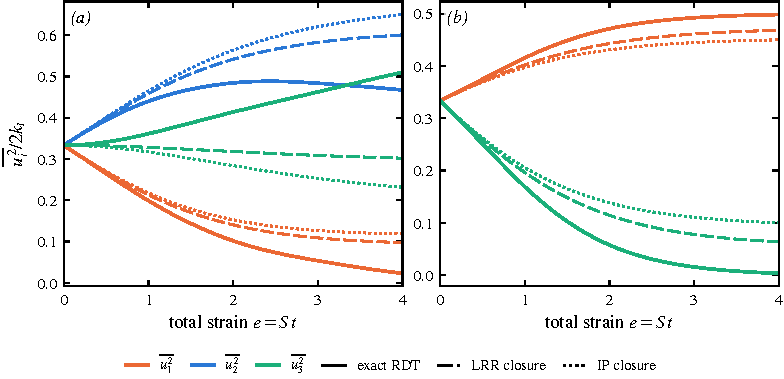
\includegraphics[width=\textwidth]{Figures/fig_rdt_components.pdf}
  \caption{Component energy fractions against total strain for initially
  isotropic turbulence under (\textit{a}) plane strain and (\textit{b})
  axisymmetric strain, normalised to $S=1$: exact rapid-distortion
  theory (wavevector-ensemble integration of \eqref{eq:rdt}) against the
  SC-ODT moment equation with the LRR closure \eqref{eq:lrr} and the IP
  closure \eqref{eq:iso-closure}. Line style denotes the source (solid
  exact RDT, dashed LRR, dotted IP) and marker the component
  ($\circ\,\overline{u_1^2}$, $\square\,\overline{u_2^2}$,
  $\triangle\,\overline{u_3^2}$). For axisymmetric strain the two
  lateral components coincide and only
  $\overline{u_1^2}=\overline{u_2^2}$ (lateral) and $\overline{u_3^2}$
  (axial) are shown. All closures share the exact onset slope; LRR
  tracks the exact solution more closely at finite strain.}
  \label{fig:rdt-components}
\end{figure}

The upwash component, whose spectrum is the input to the leading-edge
response, makes the case for the rapid term quantitative
(figure~\ref{fig:rdt-upwash}). Production acting alone drives the upwash
fraction from $1/3$ to $0.98$ by $e=4$---almost the entire kinetic
energy forced into one component, an essentially non-realisable
state---and overstates the initial amplification rate by the factor
$\tfrac52$. The rapid term removes three fifths of this at onset and
keeps the fraction physical: the exact solution peaks at $0.49$ near
$e\approx2.4$ and then relaxes as energy passes to the spanwise
component. Both closures reproduce the amplification itself---the effect
that the frozen, isotropic input of classical leading-edge-noise
prediction omits---while overpredicting it at large strain (LRR $0.60$,
IP $0.65$ at $e=4$, against the exact $0.47$). The rapid
pressure--strain is therefore necessary, and the accuracy of the method for a given configuration is controlled by the
total strain accumulated along the stagnation streamline.

\begin{figure}
  \centering
  
\includegraphics[width=0.62\textwidth]{Figures/fig_upwash_amplification.pdf}
  \caption{Upwash energy fraction under plane strain for initially
  isotropic turbulence: exact rapid-distortion theory, SC-ODT with
  the LRR and IP closures, and production alone ($B_{ij}=0$). Production
  without the rapid term overstates the onset amplification rate by
  $\tfrac52$ and forces almost all the energy into the upwash component;
  the rapid term keeps the amplification physical.}
  \label{fig:rdt-upwash}
\end{figure}

\subsection{Verification of the implementation}\label{sec:level1a}

The preceding checks verify the \emph{formulation}. They do not test the
\emph{implementation}, in which the operator is not prescribed but
reconstructed at every substep: the line Reynolds stress is formed from
the resolved field, the closure supplies $\Pi^{(\mathrm r)}_{ij}$, the
Lyapunov equation \eqref{eq:lyapunov} is solved for $B_{ij}$, and
$\mathcal{A}_{ij}=-A_{ij}+B_{ij}$ is applied pointwise. To isolate this
chain the solver is run in the rapid-distortion limit---plane strain,
eddy events suppressed, zero molecular diffusion---from a statistically
isotropic resolved initial field, and the component energies are
evaluated as length-weighted line averages. With the events inactive the
line's component-energy evolution must coincide with the closed moment
equation across the whole strain range, not merely at onset.

Figure~\ref{fig:level1a} shows that it does: the solver output lies on
the LRR trajectory over $0\le e\le4$ to within $10^{-4}$ in each
component fraction, so the per-substep stress reconstruction, Lyapunov
solve and operator assembly are correct at every state of anisotropy.
The comparison must be read correctly: the solver reproduces the
\emph{closure}, and it should---with the events suppressed the line
carries no information beyond the single-point statistics the closure
itself uses. The offset from the exact solution is the single-point
closure error of \S\,\ref{sec:finite-strain}, not an implementation
error; agreement with the exact solution here would indicate a fault.
The fractions test only the anisotropy; the kinetic energy, which the
traceless rapid term cannot change directly and which grows through the
production integral
$\mathrm{d}\ln k_t/\mathrm{d}e=f_{22}-f_{11}$, provides the independent
magnitude check, and the solver reproduces the LRR amplification to
within $0.3\%$. For definiteness: every strained computation in the
remainder of the paper uses the LRR closure, whose error against the
exact solution is quantified above at every strain reached; the
sensitivity of the spectral conclusions to this closure choice is not
estimated but measured, through the exact-RDT companions of
\S\,\ref{sec:val-spectrum} and the axisymmetry measurement of
\S\,\ref{sec:gate}, which carry the closure deficiency into the quoted
uncertainty rather than leaving it implicit. Reaching that figure required a resolved spectral
initialisation (a white-noise start places energy at the grid scale,
where mesh-adaption interpolation damps it) and a strain-resolved
timestep bound in the inviscid limit; both effects act nearly
isotropically, so the energy panel is what exposes them.

\begin{figure}[!t]
  \centering
  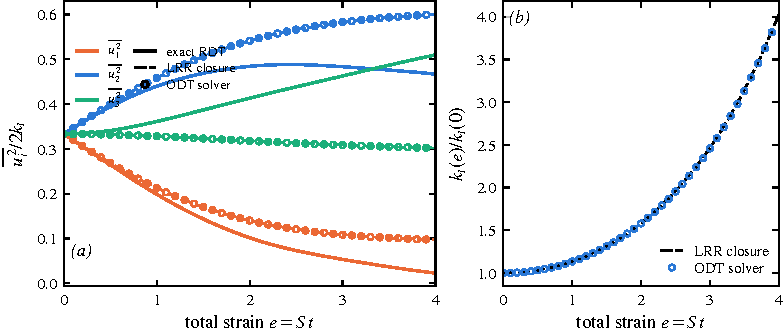
\includegraphics[width=\textwidth]{Figures/fig_level1a.pdf}
  \caption{Verification of the SC-ODT implementation under plane
  strain, eddy events suppressed and zero molecular diffusion.
  (\textit{a}) Component energy fractions; (\textit{b}) kinetic-energy
  amplification $k_t(e)/k_t(0)$. Open symbols: the SC-ODT line solver
  (length-weighted line averages), by component
  ($\circ\,\overline{u_1^2}$, $\square\,\overline{u_2^2}$,
  $\triangle\,\overline{u_3^2}$); dashed: the LRR closure integrated as
  a moment equation; solid with filled symbols: exact rapid-distortion
  theory. The solver reproduces the closure to $10^{-4}$ in the
  fractions and $0.3\%$ in the energy; the offset from the exact
  solution is the closure error of \S\,\ref{sec:finite-strain}, as it
  must be.}
  \label{fig:level1a}
\end{figure}

\subsection{Moment-level validation against the strained-turbulence DNS
of Lee \& Reynolds}\label{sec:lr-validation}\label{sec:lr-plane}

The DNS of \citet{LeeReynolds1985} is retained as a benchmark for one
specific reason: it was deliberately run at a turbulence Reynolds number
low enough ($q^4/\nu\varepsilon\lesssim100$) to be fully resolvable on a
single line, and it reports the Reynolds-stress anisotropy against total
strain for several irrotational strain modes alongside the analytic
rapid-distortion prediction---a graded, moment-level reference that the
spectral benchmarks of \S\,\ref{sec:val-spectrum} do not provide. The
same programme's later rapid-limit analysis
\citep{LeePiomelliReynolds1986} supplies the analytic reference used in
the supplementary CMK comparison; higher-Reynolds-number strained
computations exist, but the spectral role they would serve is filled
here by the dedicated strained-box DNS of \S\,\ref{sec:val-spectrum},
leaving \citeauthor{LeeReynolds1985}'s low-Reynolds-number study as the
appropriate moment-level benchmark for a fully resolved line. It is a
Stanford report rather than a journal paper, but it remains the
irrotational-strain benchmark of that programme's own later work: the
structure-based models of \citet{ReynoldsKassinos1995} and
\citet{KassinosReynoldsRogers2001} are validated against its plane-strain
and axisymmetric runs \citep{KassinosReynolds1998}. More recent direct
simulations of the same deformations at moderate Reynolds number provide
independent, journal-published comparators, and are overlaid on the
comparisons below: \citet{ZusiPerot2013} for plane strain
(figure~\ref{fig:lr-plane-fig}) and \citet{ZusiPerot2014} for
axisymmetric contraction (figure~\ref{fig:lr-axisym-fig}), both digitised
from their published anisotropy figures and shown over the strain range
they reach ($c\le1.65$). A direct simulation of the
\citeauthor{ChenMeneveauKatz2006} straining cycle
\citep{GualtieriMeneveau2010}, which reports the same variances and
pressure--strain budget as that experiment against a
Launder--Reece--Rodi closure, is discussed in the supplementary material.
The
comparison quantity is the anisotropy $b_{ij}$ against the deformation
ratio $c=\exp\int S\,\mathrm{d}t$ (so $\ln c$ is the total strain $e$ of
the present notation), computed from the single-point component
variances along the line, ensemble-averaged over $1000$ realisations;
no spectral transform is involved. Two of their strain modes are run:
plane strain and axisymmetric contraction, the line along a compressed
direction in each case, to the total strains of the DNS ($c=4$ and
$3.32$); the measured line compression agrees with $\exp(A_{22}t_f)$, $t_f$ the total straining time, to better than $0.3\%$, confirming the kinematic
fidelity of the dilatation. One parameter distinction matters for
interpretation: \citeauthor{LeeReynolds1985} characterise each run by
$S^{*}=Sq^2/\varepsilon$, which equals $2\chi$ identically since
$q^2=2k_t$---a correspondence of definitions, not a calibration---and
find the axisymmetric anisotropy
essentially independent of $S^{*}$---a parameter-free target---whereas in plane strain the unstrained component $b_{11}$ is
strongly $S^{*}$-dependent, spanning $b_{11}\approx0$ (slow) to
$+0.12$ (rapid) in the DNS.

Under plane strain (figure~\ref{fig:lr-plane-fig}) the model reproduces the
two strained components quantitatively across the whole range:
$b_{22}=+0.21$ at $c=3.86$ against $\approx+0.20$ in the DNS, and
$b_{33}=-0.20$ against $\approx-0.26$, capturing the trend and the bulk
of the magnitude. These are exactly the components the DNS identifies as
strain-rate-independent, so they constitute the robust part of the
comparison. Under axisymmetric contraction the model reproduces the
sign structure and the monotonic approach to a strained state while
under-predicting the anisotropy magnitude by roughly $25\%$
($b_{11}=-0.21$ against $\approx-0.29$ at $c=3.16$), dominated by the
spectral-closure gap isolated in \S\,\ref{sec:finite-strain} and common
to the whole second-moment family; the line adds only a small artefact,
breaking the transverse symmetry only slightly: $b_{22}=+0.102$ and
$b_{33}=+0.113$ are nearly identical, as axisymmetry requires, so the
figure plots their symmetry-respecting mean
$\tfrac12(b_{22}+b_{33})$. Figure~\ref{fig:lr-axisym-fig}
shows the comparison, with the independent DNS of \citet{ZusiPerot2014}
tracking both the model and Lee \& Reynolds over the strain range it
reaches.

\begin{figure}
  \centering
  
\includegraphics[width=0.8\textwidth]{Figures/fig_LR_plane.pdf}
  \caption{Reynolds-stress anisotropy under plane strain: SC-ODT
  (lines; ensemble mean over $1000$ realisations, standard-error band)
  against the DNS of \citet{LeeReynolds1985} (open symbols, digitised
  from their figure~5.4). Line style and marker denote the component
  ($b_{11}$ solid/$\circ$, $b_{22}$ dashed/$\square$, $b_{33}$
  dotted/$\triangle$); open markers are \citet{LeeReynolds1985}, filled
  markers the independent DNS of \citet{ZusiPerot2013} (their highest
  rate, over the strained range $c\le1.65$); the hatched band is the DNS
  $b_{11}$ range over slow-to-fast $S^{*}$. The strained components
  $b_{22}$ and $b_{33}$ are reproduced quantitatively, and the two DNS
  agree where they overlap; the unstrained $b_{11}$ is
  strain-rate-dependent in the DNS, with SC-ODT at its
  slow-strain edge.}
  \label{fig:lr-plane-fig}
\end{figure}

\begin{figure}
  \centering
  
\includegraphics[width=0.72\textwidth]{Figures/fig_LR_axisym.pdf}
  \caption{Reynolds-stress anisotropy under axisymmetric contraction:
  SC-ODT (lines; ensemble mean over $1000$ realisations) against the DNS of \citet{LeeReynolds1985} (open markers) and the
  independent DNS of \citet{ZusiPerot2014} (filled markers, their highest
  rate, over $c\le1.65$). Solid/$\square$: the compressed axial component
  $b_{11}$; dashed/$\triangle$: the transverse component
  $\tfrac12(b_{22}+b_{33})$. The model tracks the sign and monotonic
  growth of both, and the two DNS agree where they overlap.}
  \label{fig:lr-axisym-fig}
\end{figure}

The one component the model does not reproduce, the plane-strain
unstrained anisotropy $b_{11}$, is not a deficiency specific to the
model, and figure~\ref{fig:lr-b11} locates it exactly. Exact linear
rapid distortion, evaluated by the wavevector-ensemble integration of
\S\,\ref{sec:finite-strain}, gives $b_{11}$ \emph{rising} to $+0.114$
at $c=4$: although $A_{1k}=0$, the rapid pressure--strain feeds the
neutral direction---the same orientation-carried redistribution as the
spanwise growth in \S\,\ref{sec:finite-strain}. (A tempting kinematic
argument, that $\langle u_1^2\rangle$ is conserved because the
component is unstrained, holds for production but not for the rapid
term, and gives the wrong sign; an earlier version of this comparison
used it.) The fast-strain DNS therefore \emph{tracks exact RDT}, as
\citeauthor{LeeReynolds1985} themselves observed, while both
single-point closures give $b_{11}\approx0$, slightly negative: the
closure family misses the neutral-direction feed, which is carried by
the orientation distribution that single-point models discard---the
same deficiency measured spectrally, and localised in the closure's
$b$-dependent term, in \S\,\ref{sec:order}. SC-ODT
coincides with the closure on which its operator is built, so its
near-zero $b_{11}$ is correct for its formulation and matches the DNS
at slow strain rate, where the nonlinear scrambling erases the
neutral-direction feed; at fast strain it inherits the closure
family's known limitation (\S\,\ref{sec:finite-strain}) rather than any line-specific artefact.
The components that govern the upwash spectrum fed to the leading-edge
response are precisely those the model reproduces quantitatively.
Finally, \citeauthor{LeeReynolds1985}'s own transport-budget analysis
finds that in plane strain the intercomponent transfer is carried almost
entirely by the rapid term---independent support for the rapid/slow
decomposition on which \S\,\ref{sec:gate} rests.

\begin{figure}
  \centering
  
\includegraphics[width=0.82\textwidth]{Figures/fig_LR_b11_closure.pdf}
  \caption{The unstrained-direction anisotropy $b_{11}$ under plane
  strain: SC-ODT (solid, $1000$ realisations)
  against exact linear rapid distortion (long-dashed,
  wavevector-ensemble integration), the IP (dotted) and LRR-QI
  (short-dashed) closures, and the DNS of \citet{LeeReynolds1985} (open
  squares; hatched band = DNS range over slow-to-fast $S^{*}$). The
  fast-strain DNS tracks exact RDT, whose rapid pressure--strain feeds
  the neutral direction; the single-point closures---and SC-ODT, built
  on them---miss this orientation-carried redistribution, the
  deficiency measured and localised in \S\,\ref{sec:order}.}
  \label{fig:lr-b11}
\end{figure}

% =========================================================================
\section{The linear reference and the distorted spectrum}\label{sec:val-spectrum}
% =========================================================================
%% ASSEMBLED from M2 material (final-form, transplanted below) + V2
%%   sec:spec-bvc (reframed version) + a compressed CMK comparison.
%% ORDER: kinematic reference -> exact projected-RDT reference ->
%%   strain-on/off (model-internal) -> CMK (experiment, compressed) ->
%%   the strained-box DNS + three-way + envelope.
%% NOTE: labels sec:rapid-kernel, eq:rdt, sec:spec-bvc, sec:lr-plane,
%%   sec:gate referenced inside the transplants resolve once the
%%   formulation/verification transplants land.

This section establishes what SC-ODT predicts for the strained spectrum
and measures it against the correct linear reference and against DNS.
It first separates the model's own kinematics---a rigid spectral
translation---from the prediction of linear theory for the
line-projected spectrum, which is \emph{not} rigid
(\S\S\,\ref{sec:spec-rdt}--\ref{sec:spec-linref}); it then examines the
emergent distorted spectrum and fixes the physical operating point
(\S\S\,\ref{sec:spec-bvc}--\ref{sec:spec-op}); and it closes with the benchmark that addresses the model-versus-itself comparison---a
strained-box DNS with an exact rapid-distortion companion, reduced to
the same one-dimensional observables (\S\,\ref{sec:box-dns}).

\subsection{Compression without cascade: the model's kinematic
reference}\label{sec:spec-rdt}

With the eddy events suppressed and zero molecular viscosity, the mean strain
is the only process acting on the resolved field, and its effect on the line
is purely kinematic. The line length contracts as
$\mathcal{L}(e)=\mathcal{L}_0\,e^{A_{22}e}$, so every resolved wavenumber is
rescaled as $k(e)=k(0)\,e^{-A_{22}e}$---the wavevector kinematics it shares
with rapid-distortion theory \citep{BatchelorProudman1954,HuntCarruthers1990}%
---while the continuous redistribution operator of
\S\,\ref{sec:rapid-kernel} acts uniformly on every resolved wavenumber. The
combination transfers no energy between scales: a rigid translation of the
line spectrum towards higher wavenumber. This rigid translation is a property of the SC-ODT \emph{line}---uniform
dilatation composed with a wavenumber-uniform operator---and not of linear
distortion theory itself; the correct linear reference for the projected
spectrum is constructed in \S\,\ref{sec:spec-linref} below. As a check on the
implementation, however, the rigid translation is an exact, parameter-free
target.

Figure~\ref{fig:spec-rdt} confirms it. The component spectra translate toward
higher $k$ without change of shape---the peak neither broadens nor develops an
inertial range---and the spectral centroid follows
$\mathrm{e}^{-A_{22}e}$, reaching $7.03$ at $e=3.9$ against the exact
$7.03$, with the three components migrating identically; the domain
length follows $\mathrm{e}^{A_{22}e}$ to four digits. The single-point moments are
unchanged from the no-dilatation case, since a uniform rescaling of position
leaves the length-weighted velocity statistics invariant. Compression
therefore acts entirely on the spectrum and reproduces the model's kinematic
prediction exactly. It is the kinematic reference (the dashed line in all
centroid figures below) against which the full model is measured.

\begin{figure}
  \centering
  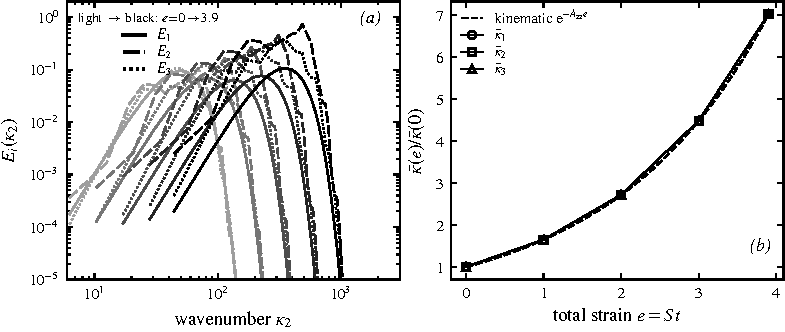
\includegraphics[width=\textwidth]{Figures/fig_spec_kinematic.pdf}
  \caption{Compression without cascade (eddy events suppressed, inviscid).
  (\textit{a}) Component line spectra $E_i(\kappa_2)$ at total strains
  $e=0,1,2,3,3.9$ (lighter to darker); the spectra translate to higher
  wavenumber without changing shape.
  (\textit{b}) Spectral-centroid migration $\bar\kappa(e)/\bar\kappa(0)$
  for each component (symbols) against the kinematic prediction
  $\mathrm{e}^{-A_{22}e}$ (dashed). The centroid follows the prediction
  and the three components coincide, confirming purely geometric
  compression of the line.}
  \label{fig:spec-rdt}
\end{figure}

\subsection{The linear reference for the projected spectrum: exact
RDT}\label{sec:spec-linref}

The rigid translation above must not be mistaken for the prediction of
linear rapid-distortion theory for the quantity the line actually carries.
In the full linear theory the amplitude of each Fourier mode evolves at a
rate that depends on the orientation of its three-dimensional wavevector
(equation~\ref{eq:rdt}); the one-dimensional component spectra are
projections---integrals over the transverse wavenumber plane---and there is
no reason for a projection of orientation-dependent amplification to
translate rigidly. Whether it does is a question of calculation, and the
answer is that it does not. Using the closed-form Cauchy solution of the
linear problem for an isotropic initial spectrum, integrated analytically
over the transverse wavenumber plane and band-limited to the wavenumbers
resolved by the DNS box of \S\,\ref{sec:box-dns}, we define the shape ratio
$R_{nn}(\kappa_2)$ as the projected component spectrum at strain $e$,
normalised by its integral, divided by the rigidly translated initial
spectrum normalised likewise; $R_{nn}\equiv1$ at every $\kappa_2$ if and
only if the translation is rigid. At $e=1$ under plane strain the upwash
ratio $R_{22}$ falls monotonically from $0.86$ at half the initial spectral
centroid to $0.36$ at ten times it: exact linear theory redistributes the
projected upwash spectrum towards low wavenumber by a factor of $2.4$
across the resolved range, because modes aligned with the line
($\kappa\to\kappa_2$) are amplified least. The transverse components are
affected more weakly ($R_{11}$ from $1.07$ to $0.81$; $R_{33}$ within seven
per cent of unity), so the projected anisotropy of linear theory is itself
scale-dependent. Figure~\ref{fig:rdt-projection} shows the ratios. The
exact-RDT companions of the DNS (\S\,\ref{sec:box-dns}), which share its
initial fields, reproduce these analytic curves to within $0.05$ in the
transverse splitting over the resolved band; the analytic integral is
used because the companions sample the largest scales with one Fourier
line per band.

\begin{figure}
  \centering
  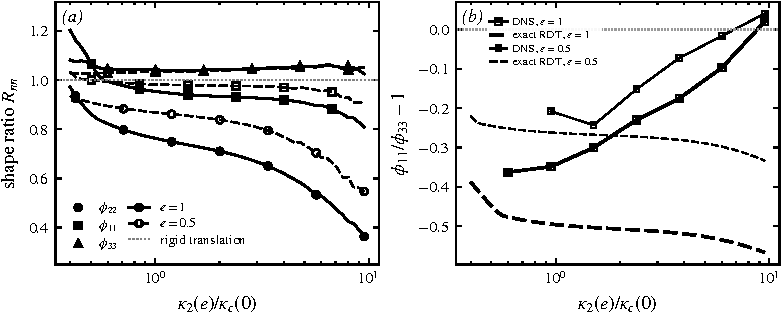
\includegraphics[width=\textwidth]{Figures/fig_rdt_projection.pdf}
  \caption{Exact linear theory does not translate the projected spectra
  rigidly. (\textit{a}) Shape ratio $R_{nn}(\kappa_2)$ of the exactly
  distorted, line-projected component spectra to a rigid translation under
  plane strain, at $e=1$ (solid, filled markers) and $e=0.5$ (dashed, open
  markers); markers distinguish the components, and the dotted line is the
  rigid translation $R_{nn}=1$. Closed-form Cauchy solution for an
  isotropic initial spectrum, integrated over the transverse wavenumber
  plane. (\textit{b}) Transverse splitting $\phi_{11}/\phi_{33}-1$ versus
  wavenumber in exact linear theory (dashed) and in the strained-box DNS of
  \S\,\ref{sec:box-dns} (solid, squares), at $e=1$ (heavy) and $e=0.5$
  (light).}
  \label{fig:rdt-projection}
\end{figure}

Two consequences run through the remainder of the paper. First, the
comparison of the full model against the rigid translation
(\S\,\ref{sec:spec-bvc}) measures the departure of the model from its own
kinematics; the departure of the \emph{flow} from linear theory must be
measured against the exact projected reference, and the two differ already
at the linear level. Second, the model's rigid spectral kinematics is
itself a structural approximation---linear theory deepens the projected
anisotropy with wavenumber, which a wavenumber-uniform operator cannot
represent---and \S\,\ref{sec:threeway} quantifies the resulting deficiency
against both the exact reference and DNS.

%% TRANSPLANTED 2026-09-07: sec:spec-bvc (reframed post-M2 version,
%%   near-verbatim) + sec:spec-Re/spec-op COMPRESSED to one operating-
%%   point subsubsection + sec:cmk compressed.  ALL underlying ensembles
%%   RERUN on caro (B5/B5off nu=1e-5 x128, OP nu=3e-6 16000 cells x256;
%%   the old WSL data are gone) and all figures rebuilt in the canon;
%%   numbers below are from the fresh ensembles.

\subsection{The distorted spectrum: strain on against strain
off}\label{sec:spec-bvc}

The central model-internal comparison isolates what the strain does to
the spectrum at fixed Reynolds number, holding the turbulence otherwise
identical. Two ensembles of $128$ realisations are run at $\nu=10^{-5}$:
SC-ODT (eddies and dilatation active) and a baseline identical
in every respect except that the strain machinery is switched off, so
the line does not compress---which is standard ODT, the $A_{ij}=0$
limit of \S\,\ref{sec:summary}. Because the two differ only in the presence
of the mean strain, the difference between them is the distortion,
cleanly separated from the cascade and dissipation the eddies produce on
their own.

Figure~\ref{fig:spec-bvc} shows the result, and it departs from the
kinematic reference in a specific and physically meaningful way.
Consider the centroid first. The no-strain baseline, after the brief
initialisation transient, relaxes monotonically to
$\bar\kappa/\bar\kappa_0<1$: with no compression, the eddies merely
redistribute energy and the centroid drifts below its initial value.
SC-ODT is lifted clearly above this baseline---compression does push
the spectrum towards higher wavenumber---yet it settles at
$\bar\kappa/\bar\kappa_0\approx1.6$--$2.1$, far below the
rigid-translation line, which rises to $7.4$ at $e=4$. The reason is
visible in the spectra: the SC-ODT spectrum is not a rigid
translation of the baseline but a \emph{broadband} distortion. It
extends to substantially higher wavenumber than the baseline---energy is carried to small scales by compression and cascade---but the
bulk of the energy remains at the energetic scales, and what reaches
high wavenumber is dissipated there rather than accumulated.

Two distinct effects are mixed in this departure, and
\S\,\ref{sec:spec-linref} requires that they be separated. The first is
the eddy cascade and dissipation, which the strain-on/strain-off
construction isolates cleanly at the level of the model. The second is
that exact linear theory itself, once projected onto the line, is
already broadband (figure~\ref{fig:rdt-projection}): part of what a
rigid-translation reference attributes to nonlinearity is present in the
linear physics. The strain-on/strain-off comparison therefore measures
what the mean strain does \emph{within the model}; how the model's
distorted spectrum stands against exact linear theory and against DNS on
the same footing is answered by the three-way comparison of
\S\,\ref{sec:threeway}. What survives either way is the qualitative
point that a frozen, rigidly strained upwash spectrum misrepresents the
distorted inflow, which motivates supplying a distorted spectrum to
Amiet's theory in place of it, in the spirit of the
rapid-distortion-modified inflow spectra of \citet{deSantana2016} but
without the frozen-shape assumption.

\begin{figure}
  \centering
  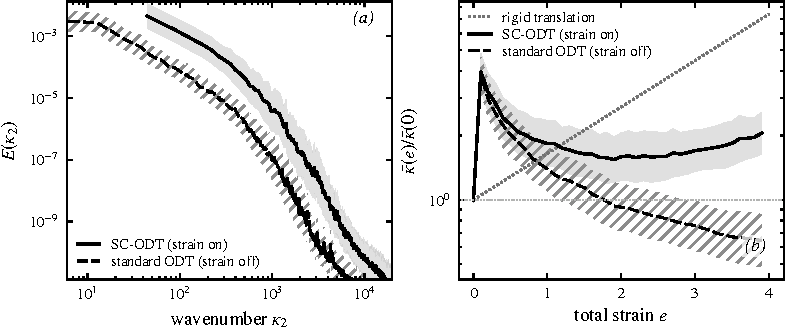
\includegraphics[width=\textwidth]{Figures/fig_spec_bvc.pdf}
  \caption{SC-ODT (strain on) against the matched strain-off baseline,
  standard ODT, at
  $\nu=10^{-5}$ (ensemble means over $128$ realisations, geometric
  $\pm\sigma$ bands). (\textit{a}) Final-strain total spectrum
  $E(\kappa_2)$: SC-ODT (strain on, solid) extends to higher wavenumber
  than the baseline (strain off, dashed) but remains broadband, not a
  rigid translation. (\textit{b}) Centroid migration: the baseline relaxes
  below unity, SC-ODT is lifted above it by the compression, yet
  stays far below the rigid-translation line (grey dotted). The gap
  between the strain-on and strain-off curves is the distortion
  attributable to the mean strain at this Reynolds number.}
  \label{fig:spec-bvc}
\end{figure}

\subsection{The physical operating point}\label{sec:spec-op}

The molecular viscosity is, in these units, the inverse integral-scale
Reynolds number, and it is a physical property of the represented
inflow, not a tunable parameter: a sweep over
$\nu=10^{-4}$--$10^{-7}$ shows the cascade deepening monotonically, with
the resolved cases settling below the linear-RDT centroid line while the
lowest viscosities climb towards it only by piling energy into an
under-resolved grid-scale shelf. The operating point is therefore the
viscosity matching the target inflow, resolution-checked. For the
reference configuration---a NACA0012 at $U_\infty=20$\,m\,s$^{-1}$ in
grid turbulence with intensity $u'/U_\infty\approx6\%$ and integral
scale $\mathcal{L}\approx55$\,mm at the leading-edge plane---the
integral-scale Reynolds number is
$Re_{\mathcal{L}}\approx4.4\times10^3$, which maps through the
initial-condition normalisation to $\nu\approx3\times10^{-6}$, run on a
refined grid ($16000$ cells) on which the dissipation rolloff is
resolved with margin; the ensemble comprises $200$ realisations.

Figure~\ref{fig:spec-op} shows the result. The component spectra fall
smoothly across four decades with no grid-scale shelf, the upwash
component $E_2$ amplified above the streamwise $E_1$---the spectral
signature of the plane strain---and no extended $k^{-5/3}$ range, as
expected physically at this Reynolds number
\citep{Kolmogorov1991,Pope2000}. The centroid settles after the
initialisation transient and migrates to $\approx2.4$ by $e=4$, far
below the rigid-translation value of $7.4$: the broadband, dissipative
distortion of \S\,\ref{sec:spec-bvc} at the physical operating point. The regime is
quantified with an estimator-free dissipation: because the eddy events
conserve energy and the production is exact, molecular dissipation is
the only sink, so it is fixed by the resolved energy budget
\begin{equation}
  \varepsilon = \mathcal{P} - \frac{\mathrm{d}k_t}{\mathrm{d}t}
              = -A_{ij}R_{ij} - \frac{\mathrm{d}k_t}{\mathrm{d}t},
  \label{eq:eps-budget}
\end{equation}
every term available on the line. By this budget the strain-rate
parameter settles at $\chi=Sk_t/\varepsilon\approx1.2$ over the strained
trajectory (ensemble of $200$ realisations), corroborated within a few
tens of per cent by the direct gradient estimate
$\langle2\nu(\partial u_i/\partial y)^2\rangle\approx1.1$: the
operating point sits at $\chi=O(1)$, bracketed by the two strained-box
DNS rapidities $Sk_t/\varepsilon=0.8$ and $16$ used in
\S\,\ref{sec:threeway}, the regime the leading-edge
stagnation flow occupies, where neither the rapid-distortion nor the
near-equilibrium limit applies and where improvement over linear theory is meaningful. The spectral \emph{peak} corroborates the regime reading
independently of the dissipation estimator: the energy-containing
wavenumber itself migrates far less than the rigid law, so the eddy
relaxation holds back the energy-containing range, not merely the
dissipation tail---linear theory misplaces the energy-containing
wavenumber, not only the spectral shape at high $\kappa$. The operating-point ensemble completes in a few hundred core-hours, roughly two orders of magnitude below a strained DNS ensemble at comparable Reynolds number, which permits parametric sweeps over inflow condition.

\begin{figure}
  \centering
  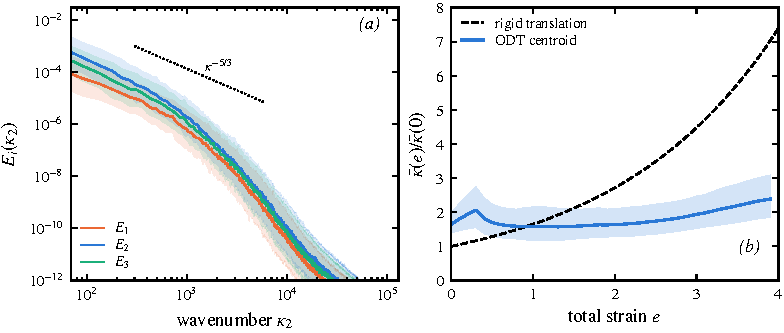
\includegraphics[width=\textwidth]{Figures/fig_spec_op.pdf}
  \caption{The physical operating point ($\nu\approx3\times10^{-6}$,
  $Re_{\mathcal{L}}\approx4.4\times10^3$, $16000$ cells; ensemble over
  $200$ realisations, geometric $\pm\sigma$).
  (\textit{a}) Final-strain component spectra (solid $E_1$, dashed
  $E_2$, dotted $E_3$): smooth rolloff with no grid-scale shelf; the
  upwash $E_2$ amplified above the streamwise $E_1$; grey dotted
  reference slope $\kappa^{-5/3}$.
  (\textit{b}) Migration of the total-spectrum centroid (solid) and the
  spectral peak (dashed) against the rigid-translation law (grey dotted), with the geometric $\pm\sigma$ ensemble spread shaded: the broadband distortion that linear theory cannot represent, at the
  operating point and with the noise averaged out.}
  \label{fig:spec-op}
\end{figure}

\subsection{Validation against a laboratory strained-turbulence experiment}\label{sec:cmk}
%% MOVED TO ESM (task U3, 2026-09-09): full text + fig_cmk_rdt +
%%   fig_cmk_aniso now in supplementary.tex \S S1; this is the summary.

The strain-on/strain-off comparison is model-internal; an external
benchmark at laboratory Reynolds number is provided by the plane-strain
experiment of \citet{ChenMeneveauKatz2006} (CMK), whose straining phase
(total deformation $D\approx3$, $e\approx2.20$ in the present notation)
we reproduce. In the rapid-distortion limit (eddy events suppressed,
inviscid) the model follows the analytic reference of
\citet{LeePiomelliReynolds1986} that CMK use---component centroids on
the rigid-translation law with deformation ratio $3.00$ at $e=2.20$,
kinetic-energy amplification $1.72$ against the exact $1.69$, the residual attributed to the moment closure, not the implementation (\S\,\ref{sec:level1a}). With eddies and viscosity active the component
centroids diverge under strain---streamwise migration $1.9$ against
$1.5$ for the upwash at the end of the straining phase, both far below
the rigid value $3$, the upwash held back most---which is the
qualitative departure-from-RDT behaviour CMK report and the spectral
signature of the broadband distortion of \S\,\ref{sec:spec-bvc}. The
comparison is qualitative by construction (initial spectrum, spectral
projection and scale separation all differ from the experiment's); the
full account, with both figures and the stated limits, is given in the
supplementary material (\S\,S1), and the quantitative spectral
assessment is carried out against the strained-box DNS below, where
projection and initial spectrum are matched by construction.

\subsection{Validation against a strained-box DNS with an exact-RDT
companion}\label{sec:box-dns}

The comparisons above are either model-internal
(\S\,\ref{sec:spec-bvc}) or, where external, qualitative by construction
(\S\,\ref{sec:cmk}) or at the Reynolds-stress level
(\S\,\ref{sec:lr-validation}). The referent quantity for the
leading-edge application is spectral, and the objection that the
emergent-spectrum results compare the model only with itself must be met
with an independent, projection-matched spectral benchmark under the
same strain. To that end
we performed direct numerical simulations of plane-strained homogeneous
turbulence in a deforming-frame (Rogallo-type) pseudo-spectral formulation:
a $128^3$ box, decaying isotropic precursor, then plane strain
$A=S\,\mathrm{diag}(\tfrac12,-\tfrac12,0)$ applied at strain-rate
parameters $Sk_t/\varepsilon\in\{0.8,16\}$ at onset, carried to total
strain $e=1$, four independent realisations
($\kappa_{\max}\eta\approx0.76$ at $e=1$: a pilot resolution, so
small-scale statements below are qualitative). Alongside every DNS
realisation runs an \emph{exact-RDT companion}: the same initial field
evolved under the closed-form Cauchy solution of the linearised equations
and projected onto lines identically to the DNS and to ODT. The companion
is what \S\,\ref{sec:spec-linref} used to construct the linear reference;
here it completes a three-way comparison in which model, linear theory and
DNS are reduced to the same one-dimensional observables. On the ODT side
the ensembles use an unstrained precursor: the line is evolved as ordinary
ODT until the initialisation transient has relaxed and the eddy population
is statistically active, and the strain is switched on only then, so that
the strained evolution starts from a physically conditioned state rather
than from the synthetic initial condition. All ODT statistics in this
subsection are medians over $1024$ realisations per case with bootstrap
confidence intervals; median statistics are used because the strained band
energies are strongly intermittent across realisations, and ensemble means
of spectral ratios are dominated by rare events at any practical sample
size.

\subsubsection{Three-way spectral anisotropy: SC-ODT, exact RDT,
DNS}\label{sec:threeway}

The comparison quantity is the strain-induced change of the spectral
component anisotropy,
$\Delta b_{nn}(\kappa_2)=\phi_{nn}/\sum_m\phi_{mm}-\tfrac13$ at strain $e$,
minus the same quantity evaluated in the system's own unstrained state with
each mode mapped to its strained wavenumber. Referencing each system to its
own $e=0$ state cancels viscous decay, which is component-blind, and the
longitudinal--transverse structure of the isotropic line spectra, which
differs between a three-dimensional box and the component-symmetric ODT
line. Figure~\ref{fig:threeway} and table~\ref{tab:threeway} give the
result at $e=1$, $Sk_t/\varepsilon=0.8$, on common bands of
$\kappa_2(e)/\kappa_c(0)$ with $\kappa_c$ the initial spectral centroid.

\begin{table}
  \centering\small
  \begin{tabular}{lccccccc}
  $\Delta b_{22}(\kappa_2)$, band $\kappa_2/\kappa_c$: & 0.5--0.75 & 0.75--1.2 & 1.2--1.9 & 1.9--3 & 3--4.8 & 4.8--7.6 & 7.6--12\\[2pt]
  exact projected RDT & $+0.146$ & $+0.008$ & $-0.020$ & $-0.041$ & $-0.050$ & $-0.054$ & $-0.056$\\
  DNS                 & $+0.032$ & $-0.033$ & $-0.029$ & $-0.032$ & $-0.036$ & $-0.040$ & $-0.046$\\
  SC-ODT              & $+0.103$ & $+0.103$ & $+0.096$ & $+0.073$ & $+0.075$ & $+0.079$ & $+0.076$\\
  \end{tabular}
  \caption{Strain-induced upwash anisotropy per wavenumber band at $e=1$,
  $Sk_t/\varepsilon=0.8$, each system referenced to its own unstrained
  state. The band below $0.75\,\kappa_c$ rests on a few box modes, so those results are indicative only.}
  \label{tab:threeway}
\end{table}

Exact linear theory concentrates
the strain-induced upwash anisotropy at the energy-containing scales and
\emph{removes} it from the small scales, because modes aligned with the
line are amplified least; the DNS shows the same shape, weakened at the
large scales by the nonlinear return---that nonlinear effects absent from
linear theory shape the strained anisotropy across scales is likewise the
finding of the $4096^3$ axisymmetric-contraction simulations of
\citet{ClayYeung2016}. SC-ODT distributes
its moment-level anisotropy essentially uniformly over wavenumber---the
signature, anticipated in \S\,\ref{sec:spec-linref}, of a
wavenumber-uniform redistribution operator acting on a uniformly dilated
line. The integrated anisotropy is nevertheless correct (the model tracks
the closure at the moment level, \S\,\ref{sec:lr-plane}), so the deficiency
is one of allocation across scales, not of amount. The transverse
splitting $\phi_{11}/\phi_{33}-1$ (figure~\ref{fig:threeway}\textit{d})
carries the same reading in a purely transverse observable: exact RDT
deepens it with wavenumber and the DNS relaxes it towards zero at the
small scales, whereas SC-ODT holds it essentially constant---the
wavenumber-uniform signature again, now in the neutral-to-streamwise
balance rather than the upwash. For the leading-edge
application the operative consequence is that the high-wavenumber
anisotropy of the upwash spectrum, which the Amiet response weights, has
the wrong sign in SC-ODT; the closure element that must carry
the correction---a wavenumber-dependent rapid operator in place of the
uniform one---is exactly the spectral kernel formulation of
\S\,\ref{sec:gate}, whose exercise is thereby motivated by this measured deficit.

\begin{figure}
  \centering
  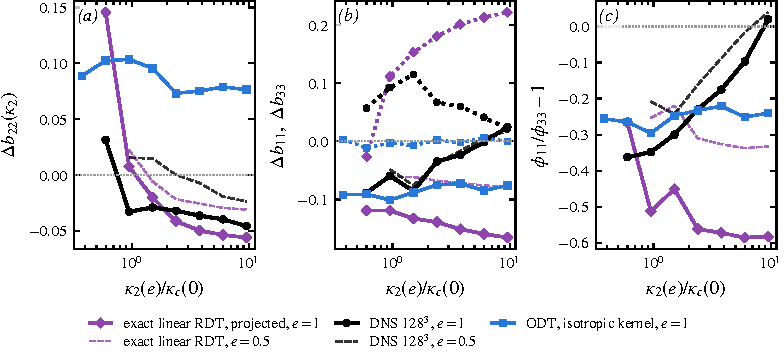
\includegraphics[width=\textwidth]{Figures/fig_threeway.pdf}
  \caption{Three-way comparison at $e=1$, $Sk_t/\varepsilon=0.8$:
  strain-induced anisotropy of the line spectra relative to each system's
  own unstrained state, resolved by component---(\textit{a})
  $\Delta b_{22}$, (\textit{b}) $\Delta b_{11}$, (\textit{c})
  $\Delta b_{33}$, (\textit{d}) the transverse splitting
  $\phi_{11}/\phi_{33}-1$. SC-ODT ($\blacksquare$, $1024$ realisations)
  against exact projected RDT ($\blacklozenge$) and DNS ($128^3$,
  $\bullet$, four realisations). The SC-ODT curves are near-flat in every
  panel---the wavenumber-uniform signature---whereas exact RDT and the DNS
  vary with wavenumber.}
  \label{fig:threeway}
\end{figure}

\subsubsection{Distance from linear theory as a function of strain
rapidity}\label{sec:envelope}

The three-way comparison resolves the anisotropy by wavenumber at one
strain-rate parameter. A complementary scalar measure tracks the
\emph{whole} spectral shape across strain and strain rapidity: at each
total strain the median ODT component line spectra are fitted, jointly in
the upwash and transverse components, by the exactly distorted spectrum of
linear theory---the closed-form Cauchy distortion of an isotropic von
K\'arm\'an field, projected onto the line, with only the pre-distortion
amplitude and energy wavenumber free. The root-mean-square log-residual of
that two-parameter fit is a scale-resolved distance between the model's
strained spectra and exact linear theory. Figure~\ref{fig:rdt-distance}
shows it for precursor-conditioned ensembles at $Sk_t/\varepsilon\approx0.4$
and $\approx8$ at onset ($1024$ realisations each, identical precursor
state: the two fits coincide at $e=0$ at thirteen per cent, the residual
shape mismatch of a relaxed ODT line against the von K\'arm\'an form).

The distance grows with strain in both cases, but \emph{faster at rapid
strain}: to approximately $22$ per cent at $e=2$ for
$Sk_t/\varepsilon\approx0.4$ against approximately $24$ per cent,
saturating early, at $Sk_t/\varepsilon\approx8$, with the separation
established already by $e=0.5$. If the model's rapid response were
spectrally faithful, the rapid curve is the one that should approach zero:
eddy events are subdominant there by construction. That the deviation is
largest where the eddies matter least localises the deficiency in
the rapid kinematics themselves---the wavenumber-uniform operator and the
rigid dilatation---and not in the eddy or relaxation statistics, in
quantitative agreement with the three-way comparison. This measured
validity envelope accompanies the model into any application: predictions
inherit a spectral-shape uncertainty of order the plotted distance at the
operating point's strain and rapidity.

\begin{figure}
  \centering
  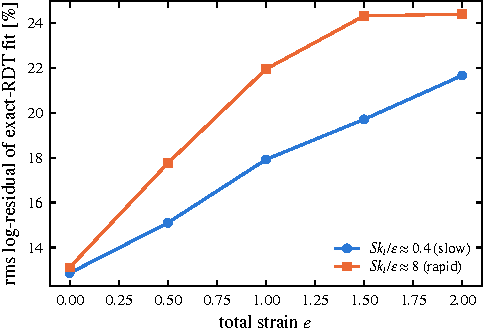
\includegraphics[width=0.62\textwidth]{Figures/fig_rdt_distance.pdf}
  \caption{Scale-resolved distance between the strained SC-ODT line spectra
  and exact linear theory: rms log-residual of the two-parameter
  exact-RDT-distorted von K\'arm\'an fit, against total strain, for slow
  and rapid onset strain-rate parameters (medians over $1024$
  realisations; identical precursor state at $e=0$).}
  \label{fig:rdt-distance}
\end{figure}

% =========================================================================
\section{Closure of the rapid pressure--strain term on a single line}\label{sec:gate}

The results of \S\,\ref{sec:val-spectrum} establish what SC-ODT
produces and where it stands against exact linear theory and DNS. The
rapid pressure--strain redistribution that drives that evolution was
evaluated throughout by the algebraic moment closure of
\S\,\ref{sec:formulation} \citep{LaunderReeceRodi1975}, applied component by
component on the resolved line. That closure is a modelling input, and the
redistribution it represents is, in its exact form, a \emph{nonlocal,
three-dimensional} object: the rapid pressure at a point is a volume
integral over the entire fluctuating field, and the pressure--strain
correlation is an integral over the full three-dimensional spectrum---one
that can be evaluated scale by scale only where the whole field is
available, as \citet{ClayYeung2016} do in a $4096^3$ simulation of
axisymmetric contraction, separating its rapid and slow parts spectrally.
What a
single one-dimensional line of turbulence can say about such an object is
the analytical question of this paper, and this section answers it short of a closure claim: we state exactly what obstructs a single-line representation, we
derive sharp bounds on the rapid term from line data alone, we
\emph{measure} rather than assume the axisymmetry hypothesis under which
the term collapses, and we identify---by measurement---which physical
content the moment closure discards.

The section proceeds as follows. The exact term and the obstruction are
stated first (\S\,\ref{sec:exact-pi}--\S\,\ref{sec:obstruction}); the
axisymmetric collapse follows, together with the statement of what it does
\emph{not} deliver (\S\,\ref{sec:assumption}); the bounds that line data do
deliver, with their falsifiers, come next (\S\,\ref{sec:bounds}); the
axisymmetry assumption is then measured directly in the strained-box DNS,
including a control experiment that isolates its failure mode
(\S\,\ref{sec:a1meas}); the component-ordering deficiency raised by the
exact solution is measured and localised (\S\,\ref{sec:order}); the
reduction to the moment closure and the disjointness from the eddy
redistribution close the argument
(\S\,\ref{sec:lrr-reduction}--\S\,\ref{sec:doublecount}).

\subsection{The exact rapid pressure--strain term}\label{sec:exact-pi}

The starting point is the Poisson equation \eqref{eq:poisson} for the
fluctuating pressure, whose source splits into a part linear in the
fluctuations and the mean velocity gradient (the \emph{rapid} part) and a
part quadratic in the fluctuations (the \emph{slow} part)
\citep{Pope2000}. The rapid part is linear in $\boldsymbol{u}'$ and
proportional to the mean gradient, which for the present homogeneous
plane strain is the constant tensor $A_{kl}$. Writing
$p'_{\mathrm r}$ for the rapid pressure and inverting the Laplacian with the
free-space Green's function $G(\boldsymbol{x})=-1/4\pi|\boldsymbol{x}|$,
\begin{equation}
  p'_{\mathrm r}(\boldsymbol{x})
  = \frac{\rho}{2\pi}\,A_{kl}\!\int
    \frac{1}{|\boldsymbol{x}-\boldsymbol{x}'|}\,
    \frac{\partial u'_l}{\partial x'_k}(\boldsymbol{x}')\,
    \mathrm{d}\boldsymbol{x}' .
  \label{eq:prapid}
\end{equation}
The rapid pressure--strain correlation that redistributes energy among the
Reynolds-stress components is
$\Pi^{(\mathrm r)}_{ij}
   = \overline{(p'_{\mathrm r}/\rho)\,(\partial u'_i/\partial x_j
     + \partial u'_j/\partial x_i)}$.
Substituting \eqref{eq:prapid} and using homogeneity to pass to the
velocity spectrum tensor
$\Phi_{mn}(\boldsymbol{\kappa})$
(the Fourier transform of $\overline{u'_m(\boldsymbol{x})\,
u'_n(\boldsymbol{x}+\boldsymbol{r})}$),
one obtains the standard exact result
\citep{BatchelorProudman1954,Crow1968,HuntCarruthers1990}
\begin{equation}
  \Pi^{(\mathrm r)}_{ij}
  = A_{kl}\,M_{ijkl},
  \qquad
  M_{ijkl}
  = \int_{\mathbb{R}^3}
    \Bigl[\,
      \frac{\kappa_j\kappa_k}{\kappa^2}\,\Phi_{il}(\boldsymbol{\kappa})
      + \frac{\kappa_i\kappa_k}{\kappa^2}\,\Phi_{jl}(\boldsymbol{\kappa})
    \,\Bigr]\,\mathrm{d}\boldsymbol{\kappa},
  \label{eq:Mijkl}
\end{equation}
where $\kappa=|\boldsymbol{\kappa}|$. Equations
\eqref{eq:poisson}--\eqref{eq:Mijkl} are exact; no modelling has entered. The
tensor $M_{ijkl}$ is a linear functional of the \emph{full three-dimensional}
spectrum $\Phi_{mn}(\boldsymbol{\kappa})$ through the nonlocal projection
operator $\kappa_a\kappa_b/\kappa^2$, which is the wavenumber-space image of
the inverse Laplacian in \eqref{eq:prapid}. This nonlocality and
three-dimensionality are the obstruction that the single-line model must
confront.

\subsection{The obstruction: what an ODT line resolves}\label{sec:obstruction}

ODT evolves a velocity vector $\boldsymbol{u}'(y)$ on a single line aligned
with the resolved direction, here taken along the contraction axis of the
strain, $y\equiv x_2$. From it the model has access to the one-dimensional
spectra
\begin{equation}
  \phi_{mn}(\kappa_2)
  = \int_{\mathbb{R}^2}
      \Phi_{mn}(\boldsymbol{\kappa})\,
      \mathrm{d}\kappa_1\,\mathrm{d}\kappa_3,
  \label{eq:phi1d}
\end{equation}
the one-dimensional spectra obtained by integrating $\Phi_{mn}$ over the two
unresolved wavenumber components. The integrand of \eqref{eq:Mijkl}, by
contrast, carries the \emph{direction-resolved} weight
$\kappa_a\kappa_b/\kappa^2$, which cannot be reconstructed from
$\phi_{mn}(\kappa_2)$ alone: integrating out $\kappa_1,\kappa_3$ as in
\eqref{eq:phi1d} destroys exactly the angular information that the projection
operator acts on. The reduction $M_{ijkl}\!\to\!$ (functional of
$\phi_{mn}$) is therefore not available without an assumption about how the
energy is distributed over the unresolved wavevector directions. This is the crux of the present question; we state the required assumption explicitly.

The obstruction just stated does not disappear under any symmetry
assumption short of full isotropy. As \S\,\ref{sec:assumption} shows,
axisymmetry about the line reduces the unknown spectrum to two scalar
functions of $(\kappa_2,\kappa_\perp)$---but the line data are two weighted
$\kappa_\perp$-integrals of those functions per resolved wavenumber, so the
map from what the line carries to what the rapid term requires retains an
infinite-dimensional null space. Stating this null space exactly, and
extracting what survives it, is the correct formulation of the single-line
question.

\subsection{The closure assumption and the collapsed form}
\label{sec:assumption}

\paragraph{Assumption A1 (axisymmetry of the undistorted spectrum about the
line).} The spectrum tensor of the incoming turbulence, before the rapid
distortion acts, is axisymmetric about the resolved direction $\boldsymbol{e}_2$:
$\Phi_{mn}(\boldsymbol{\kappa})$ depends on $\boldsymbol{\kappa}$ only through
$\kappa_2$ and $\kappa_\perp=(\kappa_1^2+\kappa_3^2)^{1/2}$, and its
polarisation is invariant under rotation about $\boldsymbol{e}_2$.

This is a statement about the \emph{turbulence}, not about the strain. It is
justified for the present configuration because the inflow is grid turbulence,
which is closely isotropic at the grid and is subsequently contracted along a
single axis as it approaches the stagnation plane; isotropy is the special
case of A1, and uniaxial contraction preserves axisymmetry about the
contraction axis. The plane strain $A_{kl}=\mathrm{diag}(\tfrac12,-\tfrac12,0)$
acting at the leading edge is itself \emph{not} axisymmetric, so A1 is imposed
on the state on which the rapid operator acts, consistent with the
rapid-distortion ordering in which $\Pi^{(\mathrm r)}$ is evaluated on the
current (here, axisymmetric to leading order) field. The error incurred when
the accumulated distortion has driven the spectrum away from axisymmetry is
quantified in \S\,\ref{sec:a1meas}.

Under A1 the angular integral in \eqref{eq:Mijkl} can be carried out. Writing
$\boldsymbol{\kappa}=(\kappa_\perp\cos\theta,\ \kappa_2,\
\kappa_\perp\sin\theta)$ and using that, by A1, $\Phi_{mn}$ is independent of
$\theta$, the azimuthal averages of the projection weights reduce to
\begin{equation}
  \Bigl\langle \frac{\kappa_1^2}{\kappa^2}\Bigr\rangle_\theta
  = \Bigl\langle \frac{\kappa_3^2}{\kappa^2}\Bigr\rangle_\theta
  = \frac{1}{2}\,\frac{\kappa_\perp^2}{\kappa^2},
  \qquad
  \Bigl\langle \frac{\kappa_2^2}{\kappa^2}\Bigr\rangle_\theta
  = \frac{\kappa_2^2}{\kappa^2},
  \qquad
  \Bigl\langle \frac{\kappa_1\kappa_3}{\kappa^2}\Bigr\rangle_\theta = 0,
  \label{eq:angular}
\end{equation}
with $\kappa^2=\kappa_2^2+\kappa_\perp^2$, and all weights mixing a resolved
and an unresolved index (e.g.\ $\kappa_1\kappa_2/\kappa^2$) averaging to zero.
Substituting \eqref{eq:angular} into \eqref{eq:Mijkl} removes the azimuthal
dependence and leaves a two-dimensional integral over $(\kappa_2,\kappa_\perp)$
of the axisymmetric spectrum. Defining the diagonal one-dimensional spectra
along the line,
\begin{equation}
  E_n^{\,\|}(\kappa_2)
   = \int_0^\infty \Phi_{nn}(\kappa_2,\kappa_\perp)\,
     2\pi\kappa_\perp\,\mathrm{d}\kappa_\perp
   \quad(\text{no sum}),
   \label{eq:Epar}
\end{equation}
the rapid pressure--strain term reduces to a two-dimensional integral over the
half-plane $(\kappa_2,\kappa_\perp)$ of the axisymmetric spectrum. The
axisymmetric, solenoidal spectrum is fixed by two scalar functions of
$(\kappa_2,\kappa_\perp)$ \citep{Batchelor1946,ChandrasekharAxisym1950}; we
denote them $a(\kappa_2,\kappa_\perp)$ and $c(\kappa_2,\kappa_\perp)$, where
$a$ is the isotropic-like scalar (the sole survivor when the turbulence is
isotropic) and $c$ measures the axisymmetric departure from isotropy. Carrying
out the azimuthal average \eqref{eq:angular} and specialising to the plane
strain $A=\mathrm{diag}(\tfrac12,-\tfrac12,0)$, the diagonal rapid
pressure--strain components are
\begin{equation}
  \Pi^{(\mathrm r)}_{nn}
  = \int_{0}^{\infty}\!\!\int_{0}^{\infty}
      g_{n}(x)\,\bigl[\,a(\kappa_2,\kappa_\perp),\,c(\kappa_2,\kappa_\perp)\,\bigr]\,
      2\pi\kappa_\perp\,\mathrm{d}\kappa_\perp\,\mathrm{d}\kappa_2
   \quad(\text{no sum on }n),
  \label{eq:Piclosed}
\end{equation}
with $x\equiv\kappa_2^2/\kappa^2$, $\kappa^2=\kappa_2^2+\kappa_\perp^2$, and the
kernels, linear in the two spectral scalars,
\begin{align}
  g_{1}(x) &= a\!\left(\tfrac18 + \tfrac34 x - \tfrac78 x^2\right)
            + c\,\tfrac78\,x\,(1-x)^2, \label{eq:g1}\\[2pt]
  g_{2}(x) &= -\tfrac32\,x\,\bigl[\,a\,(1-x) + c\,(1-x)^2\,\bigr],
            \label{eq:g2}\\[2pt]
  g_{3}(x) &= a\!\left(-\tfrac18 + \tfrac34 x - \tfrac58 x^2\right)
            + c\,\tfrac58\,x\,(1-x)^2. \label{eq:g3}
\end{align}
Equations \eqref{eq:Piclosed}--\eqref{eq:g3} constitute the axisymmetric collapse:
\emph{under A1, the rapid pressure--strain term is a
functional of the axisymmetric spectral scalars $a,c$ on the resolved
half-plane and the mean strain}, with no reference to the unresolved azimuthal
structure beyond what A1 fixes. The kernels satisfy two exact constraints that
verify the reduction. First, energy conservation: pressure--strain
redistributes without changing the trace, and indeed
$g_1(x)+g_2(x)+g_3(x)=0$ identically for all $x$ and for both scalars, so
$\Pi^{(\mathrm r)}_{11}+\Pi^{(\mathrm r)}_{22}+\Pi^{(\mathrm r)}_{33}=0$.
Second, the isotropic limit: setting $c=0$ with $a$ a function of $\kappa$
alone, the integral of $g_3$ over the half-plane vanishes, so
$\Pi^{(\mathrm r)}_{33}=0$---as it must, since the plane strain has no
component along $x_3$ and the isotropic rapid term is proportional to $S_{ij}$
\citep{Crow1968}. Both constraints hold identically in the derived kernels,
confirming the tensor reduction.

The status of \eqref{eq:Piclosed}--\eqref{eq:g3} must be stated precisely,
because it is here that the closure question is decided. Under A1 the rapid
term is a linear functional of the two axisymmetric scalars
$a(\kappa_2,\kappa_\perp)$ and $c(\kappa_2,\kappa_\perp)$ on the resolved
half-plane---a \emph{two-dimensional} representation, not yet a single-line
closure, since the line determines only the $\kappa_\perp$-integrals
\eqref{eq:Epar} of fixed combinations of $a$ and $c$ and not the functions
themselves. Equations \eqref{eq:Piclosed}--\eqref{eq:g3} are therefore the
\emph{collapsed form} on which any single-line statement must be built; the
single-line content itself---what the line data pin down, and how
sharply---is established next.

\subsection{What line data determine: sharp bounds on the rapid term}
\label{sec:bounds}

Under A1 the solenoidal spectrum tensor takes the two-scalar form
$\Phi_{mn}=a\,P_{mn}+c\,\xi_m\xi_n$, with $P_{mn}$ the solenoidal projector
and $\xi_m$ the projected axis direction; realisability is the pair of
pointwise conditions $a\ge0$ and $a+(1-x)\,c\ge0$ with
$x=\kappa_2^2/\kappa^2$. The line carries $\phi_{11}(\kappa_2)
=\phi_{33}(\kappa_2)$ and $\phi_{22}(\kappa_2)$: per resolved wavenumber,
two weighted $\kappa_\perp$-integrals of the two unknown functions. The
rapid term \eqref{eq:Piclosed} is linear in $(a,c)$, so its extreme values
over everything consistent with the line data, solenoidality and
realisability are obtained from a family of linear programs, one per
$\kappa_2$, yielding sharp bounds
$[\Pi^{-}_{nn},\,\Pi^{+}_{nn}]$ and a kinematic indeterminacy
$\mathcal I_n=(\Pi^{+}_{nn}-\Pi^{-}_{nn})/2k_tS$ that quantifies exactly
how much the null space costs. The forward map from $(a,c)$ to the line
spectra and the derivation of the bound kernels are given in
Appendix~\ref{app:forward}.

Calibrated on an isotropic von K\'arm\'an spectrum (with a verification
suite pinning tracelessness, the isotropic angular averages
$+\tfrac15:-\tfrac15:0$, the longitudinal--transverse relation, and the
exact $\tfrac45 k_t S_{ij}$), the indeterminacy is
\begin{center}\small
\begin{tabular}{lccc}
constraint level & $\mathcal I_{11}$ & $\mathcal I_{22}$ & $\mathcal I_{33}$\\[1pt]
line data $+$ solenoidality $+$ realisability & 0.77 & 1.28 & 0.86\\
$+$ log-Lipschitz slope cap ($\lambda=4$) & \multicolumn{3}{c}{$<5\%$ narrower}\\
$+$ polarisation cap $|c|\le\gamma a$, $\gamma=0$ & 0.34 & 0.58 & 0.24\\
\end{tabular}
\end{center}
Two features of this table matter. Smoothness assumptions buy almost
nothing: the null space is not a roughness artefact. The polarisation cap
is the lever---but \S\,\ref{sec:a1meas} shows that under strain the
effective polarisation reaches order one, so the applicable bound in the strained regime is the uncapped one.

The representation also supplies two \emph{free falsifiers} that the line
itself reports: under A1, $\phi_{11}(\kappa_2)=\phi_{33}(\kappa_2)$ at
every wavenumber (T1) and the velocity cross-spectra vanish (T2). Any
measured transverse splitting is a wavenumber-resolved violation of A1;
rather than assuming the hypothesis, the line monitors it.

\subsection{The axisymmetry hypothesis, measured}\label{sec:a1meas}

A1 is exact for the isotropic inflow and is degraded by the plane strain
itself. Rather than estimating this error perturbatively, we measure it in
the strained-box DNS of \S\,\ref{sec:box-dns}, where the full spectrum is
available: the exact azimuthal decomposition of $\Phi_{22}$ yields the true
scalars $(a,c)$, the discarded $m=2$ azimuthal residue (the direct
A1-violation measure, with isotropic sampling floor $0.133$ in this box),
and the effective polarisation $\gamma_{\rm eff}=|c|/a$.

\begin{table}
  \centering\small
  \begin{tabular}{c|cccc|cccc}
  & \multicolumn{4}{c|}{$Sk_t/\varepsilon=0.8$} & \multicolumn{4}{c}{$Sk_t/\varepsilon=16$}\\
  $e$ & $b_{22}$ & $\gamma_{\rm eff}$ & $m{=}2$ & $\tfrac{\phi_{11}}{\phi_{33}}{-}1$
      & $b_{22}$ & $\gamma_{\rm eff}$ & $m{=}2$ & $\tfrac{\phi_{11}}{\phi_{33}}{-}1$\\[1pt]
  0    & 0.003 & 0.10 & 0.133 & $+0.06$ & 0.003 & 0.10 & 0.133 & $+0.06$\\
  0.5  & 0.064 & 0.79 & 0.166 & $-0.20$ & 0.070 & 1.28 & 0.247 & $-0.21$\\
  1    & 0.125 & 1.44 & 0.189 & $-0.32$ & 0.124 & 4.22 & 0.396 & $-0.46$\\
  \end{tabular}
  \caption{A1 measured under plane strain ($128^3$ DNS, four realisations):
  upwash anisotropy, effective polarisation, azimuthal $m=2$ residue of
  $\Phi_{22}$ (isotropic floor $0.133$), and the on-line falsifier T1.}
  \label{tab:a1meas}
\end{table}

Three conclusions follow (table~\ref{tab:a1meas}). First, the A1 error is
\emph{not} perturbatively small in the accumulated anisotropy: the residue
grows from its floor to $0.19$ at $Sk_t/\varepsilon=0.8$ and to $0.40$ at
$16$ by $e=1$---larger at rapid strain, because at moderate strain rate the
nonlinear dynamics restore axisymmetry as fast as the strain destroys it.
An $O(b^2)$ error estimate, which the symmetric structure of the discarded
harmonic suggests, is superseded by this measurement. Second, the
polarisation cap that narrows the isotropic bounds is illegitimate under
strain: $\gamma_{\rm eff}$ passes unity by $e\simeq0.5$. Third,
correspondingly, the uncapped bound brackets the exact rapid term
(evaluated by direct integration in the DNS) up to $e\approx0.25$--$0.5$
and fails beyond, and the failure is A1's, not the estimator's.

The evidence for that attribution is a control experiment: the
same box under \emph{axisymmetric contraction} with matched $A_{22}$, for
which A1 is exact by symmetry. There the $m=2$ residue stays at the
sampling floor and the transverse splitting at zero at every strain up to
$e=1$ even at $Sk_t/\varepsilon=16$, while under plane strain both grow
(figure~\ref{fig:a1control}). The single-line closure is therefore
\emph{exact for axisymmetric distortion}; its plane-strain error is a
strain-geometry property, now quantified, rather than a defect of the line
representation. For the applications: a rounded,
three-dimensional stagnation region imposes an axisymmetric strain (closure
exact); a two-dimensional leading edge imposes plane strain (closure
carries the measured correction). The acoustically relevant amplification
$b_{22}(e)$, finally, is indistinguishable between the two geometries
($0.124$ against $0.117$ at $e=1$, $Sk_t/\varepsilon=16$): the quantity the
leading-edge response consumes is robust to precisely the geometry that A1
is sensitive to.

\begin{figure}
  \centering
  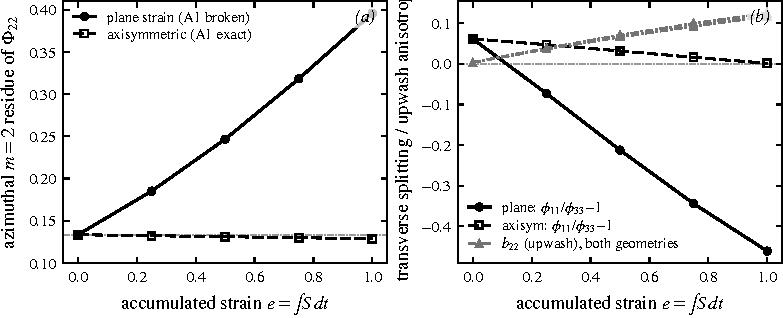
\includegraphics[width=\textwidth]{Figures/fig_a1_control.pdf}
  \caption{The A1 control experiment at $Sk_t/\varepsilon=16$ ($128^3$,
  four realisations): plane strain (A1 broken; solid, filled circles)
  against axisymmetric contraction at matched $A_{22}$ (A1 exact by
  symmetry; dashed, open squares). (\textit{a}) Azimuthal $m=2$ residue of
  $\Phi_{22}$: it grows under plane strain but stays at the isotropic
  floor (grey dotted) under axisymmetric strain. (\textit{b}) Transverse
  splitting $\phi_{11}/\phi_{33}-1$ per geometry, and the upwash
  anisotropy $b_{22}$ (grey dash-dot, indistinguishable between
  geometries)---the azimuthal structure A1 assumes away is what differs,
  while the acoustically relevant upwash amplification is robust.}
  \label{fig:a1control}
\end{figure}

\subsection{Component ordering under plane strain}\label{sec:order}

The exact solution of the rapid problem under plane strain has the neutral
spanwise component eventually overtaking the upwash; algebraic closures
predict the opposite. The exact rapid term evaluated in the DNS settles the
matter: at $e=1$, $\Pi^{(\mathrm r)}_{33}/k_tS = 0.14$ at
$Sk_t/\varepsilon=0.8$ and $0.27$ at $16$, exceeding
$\Pi^{(\mathrm r)}_{11}=0.23$ in the rapid case---the overtaking is real
and sets in at rapid strain. LRR-QI, whose spanwise component is carried by
its $b$-dependent term, matches at $Sk_t/\varepsilon=0.8$
($\Pi^{(\mathrm r)}_{33}=0.143\,k_tS$) but delivers half the exact value at
$16$; IP gives zero identically. The deficiency thus lives in the moment
closure's $b$-term, not in the line model: the ODT moment-level $b_{ij}$
follows the closure to $\sim2\%$, and its $b_{33}$ stays within $0.006$ of
zero in every run. In the spectral representation the ordering is carried
by the $c$-scalar through the kernels
\eqref{eq:g1}--\eqref{eq:g3}; the moment reduction discards it. This
answers, by measurement, where the known component-ordering error enters
and what it would take to remove it.

\subsection{Reduction to the moment closure}\label{sec:lrr-reduction}

The closed form \eqref{eq:Piclosed}--\eqref{eq:g3} operates on the resolved
spectrum, whereas the distortion results of \S\,\ref{sec:val-spectrum} were
obtained with the algebraic moment closure of \S\,\ref{sec:rapid-kernel}
\citep{LaunderReeceRodi1975}. For the two to be consistent, the spectral
kernel must reduce to that moment closure in the limit where the moment
closure is exact---isotropic turbulence. We show that it does, which both
justifies the closure used in the simulations and fixes the prefactor in an
explicit convention.

Figure~\ref{fig:pi-kernels} plots the kernels $g_1,g_2,g_3$ of
\eqref{eq:g1}--\eqref{eq:g3} against the angular variable
$x=\kappa_2^2/\kappa^2$. Two features are exact and hold for both spectral
scalars. The kernels sum to zero at every $x$,
\begin{equation}
  g_1(x)+g_2(x)+g_3(x)=0 \qquad \forall x,
  \label{eq:gtrace}
\end{equation}
so the rapid term conserves turbulent kinetic energy pointwise in wavenumber,
not merely in the integral; and each kernel vanishes at $x=1$, where the
wavevector aligns with the line and the projection $\kappa_a\kappa_b/\kappa^2$
degenerates. The signs are physically ordered: $g_1>0$ (energy fed to the
streamwise component $E_1$), $g_2<0$ (energy removed from the line/upwash
component $E_2$) over the bulk of the angular range, with $g_3$ changing sign,
consistent with the plane strain stretching $x_1$ and compressing $x_2$.

For \emph{isotropic} turbulence the anisotropy scalar vanishes ($c=0$) and the
isotropic-like scalar $a$ depends only on $\kappa$. Averaging the kernels over
solid angle---equivalently, integrating $g_n(x)$ against the isotropic
distribution of $x$ on the sphere---gives
\begin{equation}
  \langle g_1\rangle : \langle g_2\rangle : \langle g_3\rangle
  = +\tfrac15 : -\tfrac15 : 0,
  \label{eq:giso}
\end{equation}
in the ratio $+1:-1:0$. This is exactly the structure of the plane strain
$S_{ij}=\mathrm{diag}(\tfrac12,-\tfrac12,0)$: the rapid term is proportional to
$S_{ij}$, with $\Pi^{(\mathrm r)}_{33}=0$ because the strain has no component
along $x_3$. The spectral kernel therefore collapses, under isotropy, to the
isotropic-production form of the moment closure,
\begin{equation}
  \Pi^{(\mathrm r)}_{ij}
  = \tfrac{4}{5}\,k_t\,S_{ij}
  \qquad(\text{isotropic limit}),
  \label{eq:crow-spectral}
\end{equation}
the result of \citet{Crow1968} that underlies the isotropisation-of-production
(IP) rapid term in the closure of \citet{LaunderReeceRodi1975}. We note a
convention: with the symmetrised definition of the pressure--strain correlation
adopted here and the factor of two carried in the Poisson source
\eqref{eq:poisson}, the kernels \eqref{eq:g1}--\eqref{eq:g3} yield the
coefficient $\tfrac25 k_t$ for the $11$-component directly (since $S_{11}=\tfrac12$),
equivalent to the standard $\tfrac45 k_t S_{ij}$ of \eqref{eq:crow-spectral}; the ratio
\eqref{eq:giso} and the tracelessness \eqref{eq:gtrace} are independent of this
convention.

The consequence is that the algebraic closure used to obtain the distortion of
\S\,\ref{sec:val-spectrum} is not an independent assumption but the
isotropic-limit reduction of the line-consistent spectral term derived here.
The spectral form \eqref{eq:Piclosed} carries, in addition, the angular
($x$-dependent) and anisotropy ($c$-scalar) information that the moment closure
discards---and both discards are now measured: the wavenumber dependence
of the linear response in the three-way comparison of
\S\,\ref{sec:threeway}, and the component ordering in
\S\,\ref{sec:order}. The moment closure and the collapsed form thus
agree to leading order, and the terms in which they depart are exactly
the measured deficiencies of \S\,\ref{sec:val-spectrum}.

\begin{figure}
  \centering
  
\includegraphics[width=0.72\textwidth]{Figures/fig_pi_kernels.pdf}
  \caption{Rapid pressure--strain closure kernels $g_1$ (circles), $g_2$
  (squares), $g_3$ (triangles) (eqs.~\eqref{eq:g1}--\eqref{eq:g3}) against
  the angular variable $x=\kappa_2^2/\kappa^2$. Solid curves: coefficient
  of the isotropic-like spectral scalar $a$; faint grey dashed curves:
  coefficient of the anisotropy scalar $c$. The kernels sum to zero at every $x$ (energy conservation,
  eq.~\eqref{eq:gtrace}) and vanish at $x=1$. Averaged over an isotropic
  spectrum they give the ratio $+\tfrac15:-\tfrac15:0$
  (eq.~\eqref{eq:giso}), recovering the isotropisation-of-production form
  $\Pi^{(\mathrm r)}_{ij}=\tfrac45 k_t S_{ij}$ \citep{Crow1968} that underlies
  the moment closure used in \S\,\ref{sec:val-spectrum}.}
  \label{fig:pi-kernels}
\end{figure}

\subsection{Consistency with the eddy redistribution: avoiding double
counting}\label{sec:doublecount}

A closed rapid term is necessary but not sufficient: it must not duplicate
redistribution already effected by the eddy events. The pressure--strain
correlation decomposes canonically into rapid and slow parts,
$\Pi_{ij}=\Pi^{(\mathrm r)}_{ij}+\Pi^{(\mathrm s)}_{ij}$, corresponding to the two source terms in \eqref{eq:poisson}. The slow part
$\Pi^{(\mathrm s)}_{ij}$ is the return-to-isotropy mechanism, quadratic in the
fluctuations and independent of the mean gradient; the eddy events in ODT,
which act on the fluctuating field without reference to $A_{kl}$, are the
model's representation of exactly this slow redistribution. The rapid part
$\Pi^{(\mathrm r)}_{ij}$, proportional to $A_{kl}$ and linear in the
fluctuations, is by construction absent from the eddy mechanism, which carries
no dependence on the mean strain. The two therefore occupy disjoint terms of
the canonical decomposition, and adding \eqref{eq:Piclosed} as an explicit
mean-strain-driven source alongside the eddies does not double-count, provided
the eddy events are calibrated to reproduce the slow return-to-isotropy in the
absence of mean strain---a condition that the no-strain baseline of
\S\,\ref{sec:spec-bvc} verifies directly, since there the centroid relaxes
under the eddies alone with no spurious rapid contribution. This argument establishes consistency at the level of the decomposition; the no-strain baseline of \S\,\ref{sec:spec-bvc} provides the direct numerical confirmation, the centroid there relaxing under the eddy mechanism alone.

The disjointness argument is now also a measured statement, from both
sides. With the strain switched off the eddy events generate no spurious
strain-like signal (the nominal-turbulence null of
Appendix~\ref{app:numerics}). Conversely, in the rapid limit
($Sk_t/\varepsilon=16$, under one eddy per line in $e\le1$) every
kernel-energy allocation rule tested---the isotropic kernel, a
strain-biased generalisation, and discrete eddy types---reproduces the
exact rapid-distortion evolution of $b_{22}(e)$ to $\pm0.003$: the rapid
term cannot be reached from inside the eddy events, and the continuous
operator carries it alone. Rapid and slow redistribution occupy disjoint
terms by construction, and now by measurement.

\subsection{Summary: what the single-line treatment establishes}
\label{sec:gate-summary}

\begin{enumerate}
\item The rapid term is exactly $A_{kl}M_{ijkl}$; its single-line
  representation is obstructed by an azimuthal null space that is stated
  exactly and survives the axisymmetric collapse at the level of the two
  spectral scalars.
\item Under A1 the term collapses to the kernel form
  \eqref{eq:Piclosed}--\eqref{eq:g3}; A1 is exact for axisymmetric
  distortion and is \emph{measured} under plane strain, where its violation
  grows with accumulated strain and with strain rapidity
  (table~\ref{tab:a1meas}).
\item Independently of A1's validity, line data bound the rapid term
  sharply; the bound is honest---and verified to bracket the exact
  term---up to $e\approx0.25$--$0.5$ under plane strain, and at all
  computed strains under axisymmetric distortion.
\item The moment closure used in the simulations is the isotropic reduction
  of the collapsed form (verified, including the exact
  $\tfrac45k_tS_{ij}$); what it discards is the wavenumber dependence of
  the linear response and the component ordering, both measured in
  \S\,\ref{sec:val-spectrum} and \S\,\ref{sec:order}.
\item Rapid and slow redistribution are disjoint: verified by the
  strain-off null and by the rapid-limit invariance of every kernel-energy
  allocation rule.
\item The acoustically relevant upwash amplification $b_{22}(e)$ is linear
  to $e=1$ and robust to the strain geometry that controls A1's validity.
\end{enumerate}

% =========================================================================
\section{Measured limits, and scale-local relaxation}\label{sec:limits}
% =========================================================================
%% WRITTEN 2026-09-06 (the compressed Kerstein arc, all six cases).
%%   Sources: LEN_Extension results_test3 (fig_klevels, klevels_table,
%%   facSweep_table, optionA_robust_table), plan doc 4a-4e; figure
%%   regenerated for the manuscript in post/closure_bound/limits/.

The envelope of \S\,\ref{sec:envelope} localises the model's spectral
deficiency in its wavenumber-uniform rapid kinematics: the strain-induced
anisotropy is allocated uniformly across scales where linear theory and
DNS concentrate it at the energy-containing range and remove it from the
fine scales. This section asks the constructive question: which mechanism
available to the model can supply the missing scale dependence? We answer
it experimentally, by a scale-resolved diagnostic and a controlled family
of interventions in the eddy mechanism, each tested at $1024$
realisations with seeds paired to a common baseline, and each either
falsified or confirmed by the same measurement. The outcome is a single
measured statement: what is missing is \emph{scale-local relaxation}, and
supplying it---at the scales of the imbalance---is both necessary and, at
moderate strain, sufficient to move the fine-scale anisotropy.

\subsection{A transmission diagnostic}\label{sec:transmission}

The configuration is a scale-diagnostic variant of the strained line: unit
strain rate (so $e=t$), an initial spectrum peaked at a wavenumber
$\kappa_p$ resolved by more than a decade of smaller scales, and two
measurement bands, $\kappa_2\in[0.6,2]\,\kappa_p$ (the energy-containing
band) and $[6,16]\,\kappa_p$ (roughly two triplet-map generations below
it, since each map compresses by a factor of three). On each band the
component imbalance is
$\mathcal A_b = E^{\|}_2(b)/\tfrac12[E^{\|}_1(b)+E^{\|}_3(b)]$, the
band-integrated upwash energy over the transverse mean; all statistics are
medians over realisations with bootstrap confidence intervals, for the
intermittency reason given in \S\,\ref{sec:box-dns}. The model's eddy and
kernel mechanisms are component-symmetric, so $\mathcal A=1$ is their
fixed point; the strain drives $\mathcal A$ up at the scales where it
deposits anisotropy, and the ratio
$\mathcal A_{\rm hi}/\mathcal A_{\rm lo}$ measures how much of the
large-scale imbalance survives transmission down the cascade.

The baseline (supplementary material, figure~S3, black; also the black
curve of figure~\ref{fig:clock}) exhibits the deficiency of
\S\,\ref{sec:threeway} in transmission form:
$\mathcal A_{\rm hi}/\mathcal A_{\rm lo}$ stays near unity out to $e=3$
($1.02$, $0.95$, $0.89$ at $e=1,2,3$)---the anisotropy injected at the
energy-containing scales crosses two map generations essentially
undiminished---and drops only at the deepest strain. The mechanism is
direct: the high band is populated by the maps of \emph{large} eddies
(one generation takes $\kappa_p$ to $3\kappa_p$, a second to $9\kappa_p$,
inside the band), so fine-scale anisotropy is delivered by large-eddy
events, not by a chain of small ones.

\subsection{Interventions: what fails and what works}\label{sec:interventions}

The complete intervention family---each case's knob, measured
fine-scale effect and reading, with the four-panel diagnostic figure
for the eddy-locked variants---is tabulated in the supplementary
material (\S\,S2, table~S1 and figure~S3); the ledger it establishes
is set out here, with the two principal figures (the relaxation clock
and the five-way benchmark) retained below. Two
families fail for instructive reasons. Acceptance gating---rejecting
accepted eddies whose post-event state remains anisotropic, at thresholds
spanning $45$ to $98$ per cent rejection---is scale-blind: at mild
thresholds the surviving eddy population reproduces the baseline
anisotropy budget in every band (the gate self-selects eddies whose
kernels were already going to do the relaxing, and the unrelaxed field
keeps generating candidates), while at the harshest threshold the model
merely drifts towards its eddy-free limit. Restricting the gate to
sub-band-scale eddies sharpens the negative result into the mechanism
statement above: removing up to $97$ per cent of small-eddy events leaves
both the fine-scale anisotropy \emph{and} the fine-scale energy
unchanged, so no acceptance-gating scheme can control transmission at
this Reynolds number. Reweighting the triplet-map images (a middle image
of relative size $\tfrac23$, which halves the compression of the
map's dominant central channel) moves one-point and energy-containing
statistics---$\mathcal A_{\rm lo}$ falls significantly and the upwash
energy fraction with it---but not the fine scales: with the image
fractions summing to one, slowing the middle channel necessarily speeds
the outer ones, and one outer image maps the energy peak directly into
the measurement band.

What works is relaxation applied \emph{at the scale of the imbalance}.
After each accepted eddy's map and kernels, the same energy-equalising
kernel procedure (\S\,\ref{sec:formulation}) is applied to each of the
three map images---the sub-interval's own triplet-map displacement shape
as the kernel, coefficients from the sub-interval's own integrals, so
that each sub-application conserves the momentum components and the total
kinetic energy exactly, with no map applied and no random numbers
drawn---and then recursively to $9$ and $27$ sub-regions. One level
($\ell/3$ for an eddy of size $\ell$) is null: for the large eddies that
feed the band, $\ell/3$ still sits above it. Two levels produce the first
statistically significant fine-scale isotropisation of the family
($\mathcal A_{\rm hi}$ from $1.43$ to $1.27$ at $e=1$, both bands'
paired contrasts individually significant), and three levels extend the
effect to deep strain: the levels that work, $\ell/9$ and $\ell/27$, are
exactly the first that reach the measured band. Band energies move by only a few per cent, the upwash energy fraction and the intermittency tails are unchanged, and the pre-strain
fine-scale floor moves towards component equality immediately
($\mathcal A_{\rm hi}$ from $0.83$ to $0.95$ at $e=0$).

Four further variants separate the candidate explanations for the one
remaining limitation, the fading of the gains beyond $e\approx3$. Tying
the recursion depth to the eddy size (subdividing while the sub-interval
remains above a near-dissipative floor, so that large eddies do
proportionally more sub-scale work) gives the gains of depth with no
reversal at the deepest strain: both bands significant at $e=1$ and the
effect retaining its sign through $e=3$. Iterating the two-level pass
three times within each event answers the amplitude hypothesis in the
negative: it is a stronger early isotropiser but overshoots at deep
strain. Delocalising the relaxation---after each eddy, applying the
kernel isotropisation in $N$ randomly placed intervals of the same size,
overlaps allowed---tests whether the \emph{location} of the events is
the limiter: $N=1$ is null, and $N=3$ is significant in both bands at
$e=1$ but acts mainly at the energy-containing scales, since the sampled
intervals inherit the eddy-size distribution and full-interval
isotropisation acts at that scale. Stacking the two ideas---the adaptive
hierarchy inside each sampled interval---is the strongest early
isotropiser of the family ($\mathcal A_{\rm hi}$ from $1.43$ to $1.26$
at $e=1$) and delivers the only significant deep-strain effect, in the
energy-containing band at $e=3.9$; yet at the fine scales and deep
strain it overshoots the depth-only variant significantly. The ledger
is then complete for every scheme locked to the eddy clock: depth sets
\emph{where} the relaxation acts and is necessary; dosage and
delocalisation raise the early gains in proportion to the total
relaxation delivered; and no eddy-locked combination---more depth, more
dosage, more events, other locations---prevents the fine-scale fade
beyond $e\approx3$. The remaining suspect is the clock itself:
relaxation acts at the eddy rate while the strain resupplies the
imbalance continuously. Whether that is fundamental or merely
structural is decided by the final intervention.

\subsection{Decoupling the relaxation clock}\label{sec:clock}

The one axis the eddy-locked family cannot test is \emph{when}
relaxation acts. We therefore give it its own clock: an independent
Poisson stream of relaxation-only events at a prescribed rate, each
event an interval drawn from the model's eddy-size distribution, placed
uniformly on the domain, and relaxed by the same conservative kernel
pass with the adaptive-depth hierarchy inside it. Because each event
acts on an interval, momentum and kinetic energy are conserved exactly
per event; because the stream has its own rate, its pacing is decoupled
from the eddy statistics entirely. The rate is matched to the
baseline's mean eddy rate, so the comparison against the eddy-locked
variants is dose-matched by construction.

The result (figure~\ref{fig:clock}) decides the question. With the
clock, the fine-scale imbalance is reduced significantly at
\emph{every} strain and the effect grows rather than fades---the paired
contrasts reach $-0.30$ (low band) and remain significant in the high
band at $e=3.9$---because a constant-rate stream keeps pace precisely
where the eddy rate could not: event-locked timing, not any per-event
property, was the deep-strain limiter. But the uncapped stream is
scale-blind and overcorrects: it also suppresses the one-point
anisotropy that the strain should produce, pulling $u_2^2/2k_t$ from
$0.58$ to $0.41$ at $e=3.9$ and thereby breaking the moment-level
behaviour validated in \S\,\ref{sec:lr-validation}. Restricting the
stream to sub-band interval sizes ($\ell\le\ell^{*}$, the scale
separating the two measurement bands) resolves the tension: the
size-capped clock---the ``clock-relaxed ODT'' of the figures---holds the
fine scales at every strain with no
fade---$\mathcal A_{\rm hi}$ at $1.30$--$1.44$ against the baseline's
$1.63$--$1.94$, contrasts significant throughout and strongest at
$e=3$---while the one-point trajectory is essentially untouched in the
moderate-strain regime ($u_2^2/2k_t$ within $0.005$ of the baseline at
$e=1$) and only mildly reduced at the deepest strain. Increasing the rate trades off predictably: four times the rate holds the fine scales harder at a proportionate one-point cost.

\begin{figure}
  \centering
  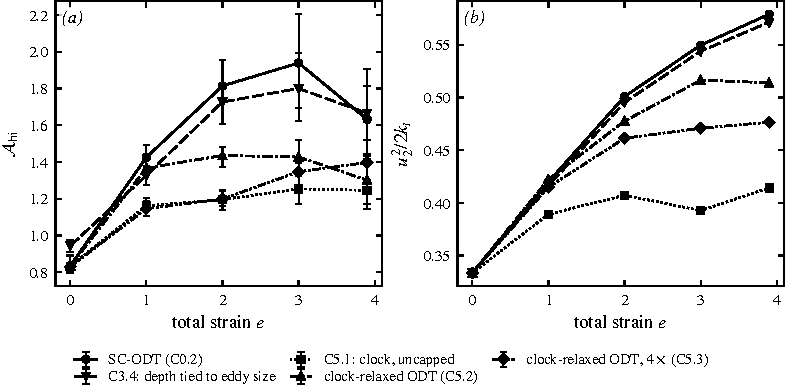
\includegraphics[width=\textwidth]{Figures/fig_clock.pdf}
  \caption{The independent relaxation clock against the eddy-locked
  family. (\textit{a}) Fine-scale-band imbalance $\mathcal A_{\rm hi}$
  against total strain: the eddy-locked variants fade beyond
  $e\approx3$; the clock holds at every strain. (\textit{b}) The
  price: upwash energy fraction---the uncapped clock suppresses the
  physical one-point anisotropy, the size cap restores it. Medians
  over $1024$ paired-seed realisations; the clock rate is matched to
  the baseline eddy rate.}
  \label{fig:clock}
\end{figure}

\subsection{The measured missing ingredient}\label{sec:limits-endpoint}

The deficiency measured by the three-way comparison---anisotropy allocated uniformly over wavenumber---is confirmed here in transmission form, is unfixable by
gating or map reweighting, and is cured by exactly two ingredients,
each isolated by a falsified alternative: relaxation applied \emph{at
the scale of the imbalance} (depth, not dosage or location) and
relaxation applied \emph{on its own clock} (the size-capped stream,
which alone survives deep strain). One limit remains, and it is structural: an isotropising mechanism is bounded at component equality and no amount of relaxation removes it, whereas exact
linear theory and the DNS carry the fine-scale upwash \emph{below} the
transverse mean. Crossing that boundary requires the rapid operator
itself to discriminate by wavenumber, and the formulation already
contains its natural form: the spectral kernel
\eqref{eq:Piclosed}--\eqref{eq:g3} is precisely a wavenumber- and
angle-dependent rapid operator, whose discretisation in place of the
wavenumber-uniform moment closure of \S\,\ref{sec:formulation} is the
identified next step.

The head-to-head that summarises this part is
figure~\ref{fig:fourway}: the strain-induced upwash anisotropy per
wavenumber band---the observable on which \S\,\ref{sec:threeway}
established the benchmark---for exact linear theory, the DNS, SC-ODT,
and the model under each of the two mechanism
forms (adaptive depth; the size-capped clock), at three strain-rate
parameters, from same-binary ensembles under the identical precursor
protocol. Four statements can be read directly from the shared axes.
First, at $Sk_t/\varepsilon=16$ the DNS lies on the exact-RDT curve:
the rapid limit is realised in the benchmark itself, and the
deficiency of the baseline model---its uniform allocation of a correct
integrated anisotropy---is starkest where the eddies matter least. Second, at moderate rapidity the mechanism tilts the model's
allocation towards the DNS---the anisotropy now decreases with
wavenumber, the fine-band excess roughly halved (at
$Sk_t/\varepsilon=0.8$: from $+0.076$ against the DNS value $-0.046$
to $+0.024$)---and the improvement grows as the rapidity falls, the
trend the application regime sits on. Third, within $e\le1$ the two
mechanism forms are equivalent on these axes; the clock's advantage is
the deep-strain hold of figure~\ref{fig:clock}, which this
protocol---bounded at $e=1$ by the DNS reference---cannot display.
Fourth, at $Sk_t/\varepsilon=16$ neither form moves the allocation:
rapid strain limits the physical time available, and no relaxation
scheme manufactures more of it. The remaining, sign-level gap belongs
to the wavenumber-dependent operator identified above.

\begin{figure}
  \centering
  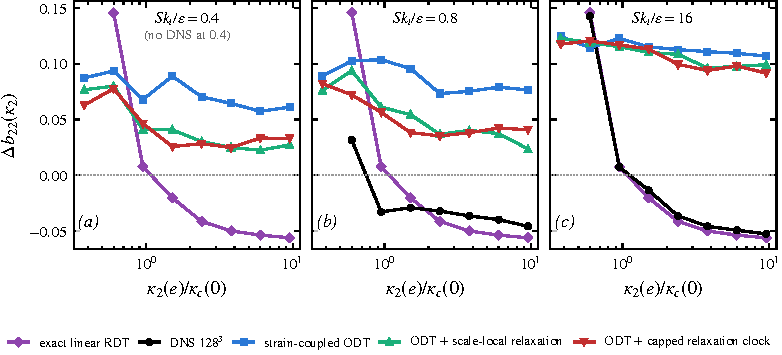
\includegraphics[width=\textwidth]{Figures/fig_fourway5.pdf}
  \caption{The five-way comparison on the benchmark observable of
  \S\,\ref{sec:threeway}: strain-induced upwash anisotropy per
  wavenumber band at $e=1$, for exact linear RDT, DNS, SC-ODT, and
  SC-ODT with each mechanism form---scale-local relaxation at adaptive
  depth, and the clock-relaxed variant (size-capped relaxation clock)---at
  $Sk_t/\varepsilon=0.4$, $0.8$ and $16$ (ODT: $1024$ realisations per
  case, same binary and precursor protocol; DNS and companions as in
  \S\,\ref{sec:box-dns}; no DNS exists at $0.4$, where exact RDT is
  the reference---at fixed total strain it is independent of the
  strain rate). At rapid strain the DNS realises the exact-RDT
  allocation; the mechanism moves the model towards the DNS
  increasingly as the rapidity falls.}
  \label{fig:fourway}
\end{figure}

% =========================================================================
\section{Consequence for leading-edge noise}\label{sec:lenoise}
% =========================================================================
%% PART III (written 2026-09-09, per the one-paper decision): the
%%   Gate-B reduction on the clean ensembles; machinery in
%%   post/closure_bound/lenoise/ (rdt_kernel validated against the
%%   Level-0 integrator to <1% in R22 growth).

The application that motivates the model can now be served with its
output. In the leading-edge-noise theory of \citet{Amiet1975} the
far-field pressure spectral density of a large-aspect-ratio aerofoil
factorises as a product of the flow and observer geometry, the aerofoil
response $|\mathcal L|^2(K_x)$, the upwash wavenumber spectrum
$\Phi_{ww}(K_x,0)$ and the spanwise correlation length
$\ell_y(K_x)=\pi\,\Phi_{ww}(K_x,0)/\!\int\Phi_{ww}(K_x,K_y)\,
\mathrm{d}K_y$, with $K_x$ the streamwise and $K_y$ the spanwise
wavenumber. For a \emph{change of inflow spectrum} at fixed aerofoil,
flow and observer, everything except the turbulence kernel
\begin{equation}
  \mathcal K(K_x)
  \;=\;
  \pi\,\frac{\Phi_{ww}(K_x,0)^2}{\int\Phi_{ww}(K_x,K_y)\,\mathrm{d}K_y}
  \label{eq:knoise}
\end{equation}
cancels exactly, so the change of radiated level is
$\Delta\mathrm{SPL}(K_x)=10\log_{10}
[\mathcal K^{\rm distorted}/\mathcal K^{\rm frozen}]$, independent of
the aerofoil geometry and response. This is a question the distortion model can be asked without importing an acoustic solver:
by how much does the prediction change when the inflow spectrum is the
\emph{computed, distorted} one instead of the frozen upstream spectrum
that standard practice prescribes?

The distorted input is taken from the model's own strained ensembles in
the representation already fitted in \S\,\ref{sec:envelope}: the
exact-RDT-distorted von K\'arm\'an family, two parameters
$(A_0,\kappa_e)$ per strain, fitted to the median line spectra of the
$1024$-realisation ensembles at $Sk_t/\varepsilon\approx0.4$ and
$\approx8$. The line data pin the resolved-wavenumber structure; the
transverse structure that \eqref{eq:knoise} requires is supplied by the
representation---this is \S\,\ref{sec:gate}'s statement about line
knowledge, operating in the application---and the representation's rms
residual, $13$--$24\%$ over the strain range (the distance envelope of
figure~\ref{fig:rdt-distance}), is the corresponding uncertainty
carried by the result. The two-dimensional spectrum follows by direct
integration of the distorted components,
$\Phi_{ww}(K_x,K_y;e)=A_0\!\int\!\Phi^{\rm RDT}_{22}
(K_x,\kappa_2,K_y;e)\,\mathrm{d}\kappa_2$, with the machinery verified
against the wavevector-ensemble integrator of
\S\,\ref{sec:finite-strain} (upwash-variance growth reproduced to
under $1\%$). The frozen baseline is the same inflow's relaxed $e=0$
state carried undistorted. The level and shape contributions are
separated: the kernel scales linearly with the upwash variance, so
dividing it out isolates the spectral reallocation, and the variance
ratio itself is taken from the measured line spectra rather than from
the fit.

\begin{figure}
  \centering
  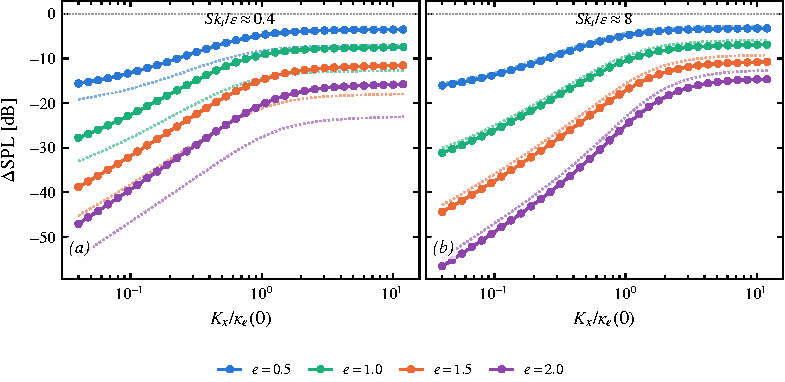
\includegraphics[width=\textwidth]{Figures/fig_lenoise.pdf}
  \caption{Change of the Amiet leading-edge-noise kernel when the
  frozen inflow spectrum is replaced by the computed distorted one,
  against reduced streamwise wavenumber, at total strains
  $e=0.5$--$2$ (shade light to dark with increasing strain):
  (\textit{a}) $Sk_t/\varepsilon\approx0.4$,
  (\textit{b}) $\approx8$. Solid: spectral reallocation at matched
  upwash variance (shape only); dotted: total, including the measured
  variance change ($-3.5$ to $-7.3$\,dB at the slow rate, where decay
  dominates the transit; $+0.5$ to $+1.9$\,dB at the rapid rate, where
  the upwash amplification survives). Geometry, aerofoil response and
  observer position cancel identically in this ratio.}
  \label{fig:lenoise}
\end{figure}

Figure~\ref{fig:lenoise} shows the result. At matched upwash variance the distorted spectrum is a
substantially \emph{weaker} leading-edge source than the frozen one at
every resolved reduced frequency: $\approx-5$\,dB at
$K_x\approx\kappa_e(0)$ for $e=0.5$, deepening to $-20$\,dB and beyond
by $e=2$, and increasingly severe towards low $K_x$. The mechanism is
the orientation physics of \S\,\ref{sec:gate} acting on the noise
kernel: \eqref{eq:knoise} weights the spanwise-coherent upwash content
$\Phi_{ww}(K_x,0)$, which lives on wavevectors aligned with the
line---exactly the orientations whose upwash is smallest by
solenoidality and whose pre-images retreat into the vanishing
low-wavenumber tail of the initial spectrum as the distortion
proceeds. The distortion therefore removes the upwash content the aerofoil responds to. The total change adds the variance term: at the
rapid rate the surviving upwash amplification offsets a small part of
the reallocation; at the slow rate viscous decay over the longer
transit deepens it.

\begin{figure}
  \centering
  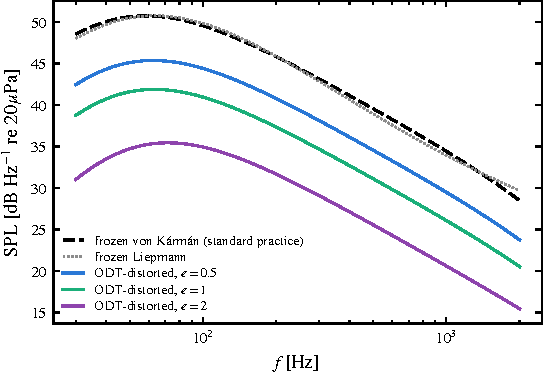
\includegraphics[width=0.7\textwidth]{Figures/fig_amiet_abs.pdf}
  \caption{The assembled absolute prediction at the reference
  configuration of \S\,\ref{sec:spec-op}: far-field sound pressure
  level from the compact lift-dipole form of \citet{Amiet1975} with
  the exact Sears response, for a flat plate of chord $0.39$\,m
  ($Re_c\approx5\times10^5$) and span $0.8$\,m at
  $U_\infty=20$\,m\,s$^{-1}$, $u'/U_\infty=6\%$,
  $\mathcal{L}=55$\,mm, observer $1$\,m overhead. Dashed: the frozen
  von K\'arm\'an inflow of standard practice (the $e=0$ member of the
  fitted representation, which is exactly the isotropic von K\'arm\'an
  spectrum); grey dotted: the frozen Liepmann spectrum at the same
  $(u',\mathcal{L})$, an independent analytic cross-check of the
  physical-unit bridge. Solid (grey light to black with increasing
  strain, circles): the same chain with the SC-ODT-distorted inflow at
  total strains $e=0.5$, $1$ and $2$
  ($Sk_t/\varepsilon\approx0.4$), level and shape both included.}
  \label{fig:amiet-abs}
\end{figure}

Figure~\ref{fig:amiet-abs} places the kernel result in the quantity
practice actually reports: the absolute far-field spectrum of the
reference configuration of \S\,\ref{sec:spec-op}, assembled from the
compact lift-dipole form of Amiet's theory with the exact Sears
response. The spectra enter in physical units through two matching
conditions only---the integral scale fixes the length unit through the
von K\'arm\'an relation $\kappa_e=0.7468/\mathcal{L}$ and the upwash
variance at $e=0$ fixes the amplitude---so the frozen baseline
\emph{is} the standard Amiet--von K\'arm\'an prediction, with no recalibration: the $e=0$ member of the representation is the
isotropic von K\'arm\'an spectrum itself, and it reproduces the
analytic one-dimensional form to within the quoted fit residual
(ratio $0.79$--$1.14$ across $100$\,Hz--$1$\,kHz), with the Liepmann
spectrum shown as an independent check of the unit bridge. Against
this baseline the computed distortion lowers the predicted level by
$5$\,dB at $e=0.5$, $9$\,dB at $e=1$ and $14$\,dB at $e=2$ across the
resolved band ($f\lesssim1.8$\,kHz at this operating point), the
spanwise-coherence drain of figure~\ref{fig:lenoise} now carried
through geometry, aerofoil response and radiation to the observer.

%% U6 (2026-09-09): experimental four-way validation; machinery in
%%   post/acoustics/{expdata,expval}; ensembles gateA_S{1,20}_RCS1.
\begin{figure}
  \centering
  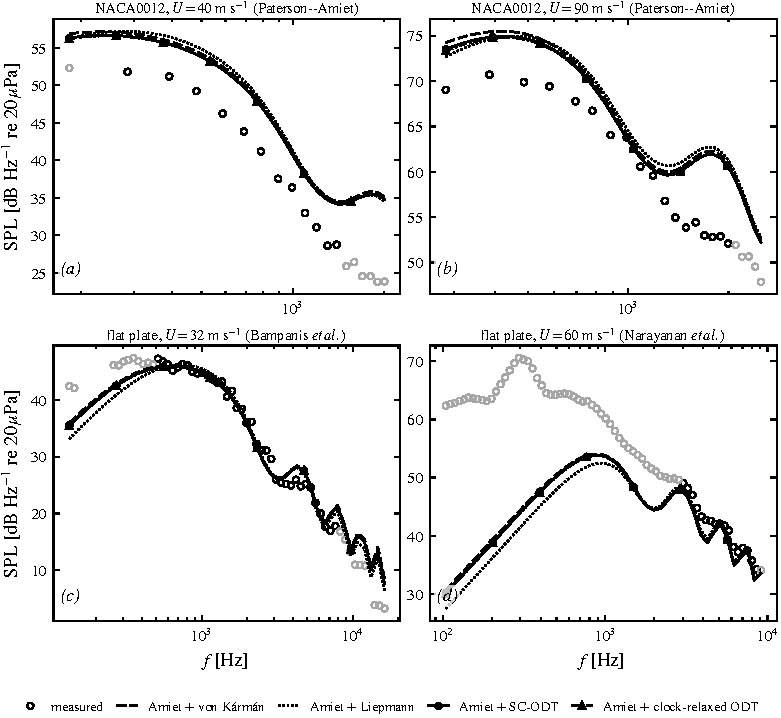
\includegraphics[width=\textwidth]{Figures/fig_expval_paper.pdf}
  \caption{Absolute far-field predictions against published
  measurements, all four inflow spectra through the identical
  non-compact response \citep{Amiet1975,RogerMoreau2010}: frozen
  von K\'arm\'an (black dashed), frozen Liepmann (grey dotted), the
  computed SC-ODT spectrum (grey, circles) and the computed
  clock-relaxed ODT spectrum (grey, triangles), each entered at the
  case's effective free-distortion strain. (\textit{a,b}) NACA0012 of \citet{PatersonAmiet1976}
  ($c=0.23$\,m, $u'_w/U\approx4$--$5\%$, $\Lambda_f\approx30$\,mm,
  observer $2.25$\,m overhead; Gershfeld thickness admittance applied
  identically to all four chains); (\textit{c}) ECL flat plate of
  \citet{Bampanis2022} ($c=0.10$\,m, $3$\,mm thick, $Tu=4.5\%$,
  $\Lambda=9$\,mm, $\Theta=90^\circ$, $R=1.25$\,m); (\textit{d}) ISVR
  flat plate of \citet{Narayanan2015} ($c=0.15$\,m, $Tu=2.5\%$,
  $\Lambda=6$\,mm, $R=1.2$\,m). Black measured symbols lie in each
  case's stated comparison band (grey outside: background flags,
  facility contamination, thickness-breakdown frequency); spectra
  digitised from the published figures with per-figure calibration
  checks ($\pm0.5$\,dB). The effective strain is a geometric estimate
  (potential-flow stagnation-line accumulation truncated at the eddy
  scale); the shaded band spans truncation at $\Lambda/4$--$\Lambda$.}
  \label{fig:expval}
\end{figure}

The chain is then confronted with measurement.
Figure~\ref{fig:expval} shows four published leading-edge-noise
experiments with fully documented inflow turbulence---the NACA0012 of
\citet{PatersonAmiet1976} at $40$--$90$\,m\,s$^{-1}$ (higher speeds
excluded only by their Mach number), and the flat plates of
\citet{Bampanis2022} and \citet{Narayanan2015}---each with four
predictions computed through the identical response: the frozen
von K\'arm\'an and Liepmann inflows of standard practice, and the
model's computed spectra, SC-ODT and clock-relaxed ODT, evaluated at the
effective free-distortion strain accumulated along the potential-flow
stagnation streamline down to the eddy scale ($e_{\rm eff}=0.09$--$0.16$
for the NACA0012; below $0.05$ for the thin plates). Three statements
result. First, the assembled chain is quantitatively right where the
experiment is cleanest: on the flat-plate cases every formulation sits
within $1$--$2$\,dB rms of the measured spectra with the
non-compactness interference lobes reproduced---the fidelity
\citet{Bampanis2022} report for their own implementation---so the
comparison discriminates inflow physics, not implementation. Second,
the computed distortion behaves causally: for the thin plates the
effective strain is negligible and the model correctly predicts
\emph{no} correction to the frozen spectrum, while for the NACA0012 it
lowers the prediction towards the data at every speed
(bias $+5.7\!\to\!+5.3$\,dB at $40$\,m\,s$^{-1}$,
$+1.8\!\to\!+1.4$\,dB at $60$, $+5.1\!\to\!+4.7$\,dB at $90$), by the
modest amount its geometric effective strain implies; the shift
between predictions is exact, since the digitisation uncertainty
($\pm0.5$\,dB) is common to all four. Third, the
SC-ODT and clock-relaxed ODT models are indistinguishable in the far
field at these laboratory strains (differences below $0.05$\,dB),
and this is stated as a limit of the test, not of the mechanism:
laboratory rigs are designed to minimise inflow distortion, so no
published far-field measurement samples the strains at which the
relaxation mechanism acts. The residual NACA0012 overprediction is
the finite-thickness effect \citet{PatersonAmiet1976} themselves
identified (breakdown near $U/f t_A\approx1$) and
\citet{Gershfeld2004} modelled, of a piece with the blocking mechanism
excluded from the present scope; it is unchanged in rank by any choice
of inflow spectrum.

\begin{figure}
  \centering
  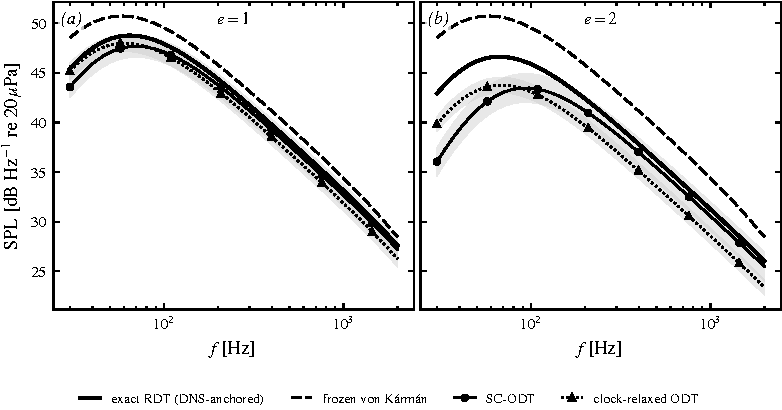
\includegraphics[width=\textwidth]{Figures/fig_amiet_rapid.pdf}
  \caption{Computed against prescribed inflow at application strains,
  judged by the linear reference: absolute SPL at the reference
  configuration for the rapid family ($Sk_t/\varepsilon\approx8$) at
  (\textit{a}) $e=1$ and (\textit{b}) $e=2$. Solid black: exact
  (inviscid) RDT of the model's relaxed initial state---the reference the
  strained-box DNS of \S\,\ref{sec:box-dns} validates at rapid
  rates---with level set by the kernel's exact upwash amplification
  (reproducing the moment-level value to $0.7\%$). Black dashed: the
  frozen von K\'arm\'an inflow of standard practice. Grey (circles:
  SC-ODT; triangles: clock-relaxed ODT): the two computed inflows
  (fitted representations, measured ensemble levels), each with a band
  giving its measured spectral rms distance from the RDT family mapped
  to decibels; the two share the band and are indistinguishable at this
  level.}
  \label{fig:amiet-rapid}
\end{figure}

Where the mechanism does reach the prediction is shown in
figure~\ref{fig:amiet-rapid}. At total strains of $1$--$2$ the frozen-spectrum
error against the linear reference grows from $+1.3$ to $+3.6$\,dB,
while both computed inflows track the reference within
$1$--$2.5$\,dB---a residual that contains the physical relaxation at
finite rapidity as well as the model deficiency measured in
\S\,\ref{sec:envelope}---so an evolved inflow improves on a prescribed one at the strains where the correction matters, whichever variant of the model evolves it. Between the two variants the
radiated \emph{level} does not discriminate: the clock acts below its
size cap, where the noise kernel carries little weight, and its gain
appears instead in the uncertainty the input carries into the
prediction---the clock-relaxed ensembles lie closer to the
exact-RDT-distorted family by a factor of two to four in rms at both
rapidities, and, unlike SC-ODT's, their distance does not
grow with strain (supplementary material, \S\,S3), which halves the
shaded band of figure~\ref{fig:amiet-rapid} and makes it
strain-independent. A far-field discrimination of the mechanism
requires a configuration whose acoustic response samples the sub-cap
scales at accumulated strains of order unity---turbulence-ingesting
rotors, where the streamtube contraction supplies the strain and the
blade response the fine-scale weighting---and is left as the
falsifiable target of the application study.

The scope is limited to the \emph{free} distortion by the mean strain: the
surface-blocking effect, which measurements and simulations show
\emph{enhancing} the near-edge upwash at low frequency
\citep{HuntGraham1978,dosSantos2023,Piccolo2024}, is a distinct and
partially compensating mechanism outside the present line model, and
the strain history along individual streamlines is replaced by the
canonical constant-rate distortion. What the calculation establishes
is the magnitude and sign of the term that frozen-spectrum practice omits: order $5$--$20$\,dB at the
energy-containing reduced frequencies for total strains of
$0.5$--$2$---of the opposite sign to the
blocking correction with which it must ultimately be combined.
Figure~\ref{fig:amiet-abs} shows that the chain from model output to absolute far-field level is complete; what remains for a
predictive comparison against measurement is the blocking correction
and the streamline strain history, for which the present model
supplies the distorted-inflow input, with its
uncertainty quantified by the envelope of \S\,\ref{sec:envelope} and
its fidelity improved by the mechanism of \S\,\ref{sec:limits}
precisely in the wavenumbers the response weights.

% =========================================================================
\section{Conclusions}\label{sec:conclusions}
% =========================================================================
%% WRITTEN 2026-09-08 (M4).  Claims mirror the abstract; no
%%   rigid-translation-as-linear-prediction claim.

We have presented a strain-coupled formulation of one-dimensional
turbulence and, around it, a systematic account of what a single line of
turbulence can and cannot say about rapid distortion. The formulation
splits the distortion physics by structure: production enters as an
exact continuous forcing, the rapid pressure--strain as an
energy-conserving operator built from an explicit spectral closure, and
the wavevector kinematics as a dilatation of the domain, while the eddy
events of the standard model continue to carry the cascade and the slow
return to isotropy. The construction preserves the model's structural
invariants, reproduces the constant-free rapid-distortion onset rate
identically, and is verified in the solver to the level of the closure
it evolves ($10^{-4}$ in the component fractions); at the moment level
it reproduces the strained components of the \citet{LeeReynolds1985}
DNS quantitatively, with the one exception---the neutral-direction
anisotropy---traced to the orientation information that every
single-point closure discards, not to the line.

Three findings shape how such a model must be judged. First, the
correct linear reference for line-projected spectra is broadband: exact
rapid-distortion theory, projected onto a line, redistributes the
projected upwash spectrum by a factor of $2.4$ across the resolved range
at $e=1$, so a rigid spectral translation---the model's own
kinematics---is not the linear prediction, and comparisons built on it
conflate a structural approximation with nonlinear physics. Second,
against a strained-box DNS with exact-RDT companions reduced to the
same observables, the strain-coupled model carries the correct
integrated anisotropy but allocates it uniformly over wavenumber, where
linear theory and DNS concentrate it at the energy-containing scales;
the deficiency is localised in the wavenumber-uniform rapid operator
and grows with strain rapidity, a measured validity envelope that
accompanies the model into any application. Third, the single-line
closure question admits an exact, falsifiable answer in place of a
closure claim: line data bound the rapid term sharply, the bounds hold up to $e\approx0.25$--$0.5$ under plane strain and at all
computed strains under axisymmetric distortion, and the axisymmetry
hypothesis is measured rather than assumed---its plane-strain violation
grows with accumulated strain and rapidity while the acoustically
relevant upwash amplification remains robust to it.

The measured limits point to a specific missing ingredient, which the
paper identifies and supplies. The strain-induced fine-scale
anisotropy is delivered directly by large-eddy maps, which is why no
acceptance-gating or map-reweighting scheme can control it; what does
move it is relaxation applied at the scale of the imbalance---the
model's own energy-equalising kernel, applied hierarchically to eddy
sub-scales. The intervention family maps the mechanism's envelope
precisely: depth that reaches the measured scales is necessary and
sufficient at moderate strain; dosage and delocalised application
raise the early gains in proportion; and the fine-scale fade beyond
$e\approx3$, common to every scheme locked to the eddy clock, is
removed by giving the relaxation its own clock---an independent stream
of relaxation events whose size cap preserves the one-point
physics. What remains is not timing but allocation: isotropisation is
bounded at component equality and cannot reach the fine-scale sign
reversal the DNS exhibits, so the remaining step is the
wavenumber- and angle-dependent spectral kernel derived in
\S\,\ref{sec:gate}; exercising it in place of the wavenumber-uniform
closure is the natural continuation, now motivated by a measured
deficit and pointed at a measured target.

For the application that motivated the work, the model delivers what
the prediction chain lacks: a distorted, anisotropic, scale-resolved
upwash spectrum, evolved rather than prescribed, at two orders of
magnitude below the cost of a strained DNS ensemble---and
\S\,\ref{sec:lenoise} carries it through Amiet's theory to the
radiated level. The assembled chain reproduces four published far-field experiments to
$1$--$2$\,dB rms where the facilities are cleanest, with the computed
correction causal---vanishing for thin plates, lowering the
prediction towards the data for the NACA0012---and, against the linear
reference at application strains, an evolved inflow improves on the frozen one by a margin that grows with strain. Relative to the
frozen-spectrum input of standard practice the computed distortion is
a weaker leading-edge source at every resolved frequency---by
$5$--$20$\,dB at the energy-containing scales for total strains
$0.5$--$2$, in the geometry-free kernel ratio and in the assembled
absolute prediction at the reference configuration alike---because the
distortion drains exactly the spanwise-coherent upwash content the
aerofoil responds to. This omitted term is opposite in sign to the surface-blocking correction with which a complete prediction must combine it; predictions inherit a spectral-shape uncertainty of order
the distance envelope at the operating point's strain and rapidity.

% =========================================================================
\appendix
\section{The forward map and the bound kernels}\label{app:forward}
%% TRANSPLANTED 2026-09-06 from notes/los_estimator_note.tex (secs 2-4),
%%   adapted to manuscript notation; kernels re-verified symbolically
%%   against A_kl M_nnkl (sympy, 2026-09-06).

This appendix derives the three ingredients that \S\,\ref{sec:gate} uses:
the two-scalar representation of the axisymmetric solenoidal spectrum with
its realisability cone, the forward map from the two scalars to the line
spectra (with the falsifiers T1--T2), and the closure kernels
\eqref{eq:g1}--\eqref{eq:g3}, together with the linear programs that turn
these linear relations into the sharp bounds of \S\,\ref{sec:bounds}.

\subsection{The axisymmetric representation and realisability}
\label{app:twoscalar}

The spectrum tensor of statistically homogeneous turbulence is Hermitian,
positive semi-definite at each $\boldsymbol{\kappa}$, and solenoidal,
$\kappa_m\Phi_{mn}(\boldsymbol{\kappa})=0$; it therefore has rank at most
two, supported on the plane normal to $\boldsymbol{\kappa}$. Under A1
(axisymmetry about $\boldsymbol{e}_2$, mirror-symmetric, helicity-free) it
is fixed by two scalar functions of $(\kappa_2,\kappa_\perp)$
\citep{Batchelor1946,ChandrasekharAxisym1950,Lindborg1995}:
\begin{equation}
  \Phi_{mn}(\boldsymbol{\kappa})
  = a(\kappa_2,\kappa_\perp)\,P_{mn}(\boldsymbol{\kappa})
  + c(\kappa_2,\kappa_\perp)\,\xi_m\xi_n,
  \qquad
  \boldsymbol{\xi} = \boldsymbol{e}_2 - \mu\,
  \frac{\boldsymbol{\kappa}}{\kappa},
  \quad \mu=\frac{\kappa_2}{\kappa},
  \label{eq:twoscalar}
\end{equation}
with $P_{mn}=\delta_{mn}-\kappa_m\kappa_n/\kappa^2$ the solenoidal
projector, so that $\kappa_m\xi_m=0$ and
$|\boldsymbol{\xi}|^2=1-\mu^2=1-x$ with $x=\kappa_2^2/\kappa^2$:
solenoidality is exact by construction, which is how the third would-be
scalar of a general axisymmetric tensor is eliminated. For a unit vector
$\boldsymbol{v}$ normal to $\boldsymbol{\kappa}$,
$\Phi_{mn}v_mv_n = a + c\,(\boldsymbol{\xi}\cdot\boldsymbol{v})^2$, so the
two eigenvalues of the polarisation matrix on that plane are $a$ (attained
for $\boldsymbol{v}\perp\boldsymbol{\xi}$) and $a+(1-x)\,c$ (for
$\boldsymbol{v}\parallel\boldsymbol{\xi}$). Positive semi-definiteness is
therefore the pointwise \emph{realisability cone}
\begin{equation}
  a(\kappa_2,\kappa_\perp)\ \ge\ 0,
  \qquad
  a(\kappa_2,\kappa_\perp) + (1-x)\,c(\kappa_2,\kappa_\perp)\ \ge\ 0 ,
  \label{eq:cone}
\end{equation}
quoted in \S\,\ref{sec:bounds}. Isotropy is the special case $c=0$ with
$a$ a function of $\kappa$ alone.

\subsection{The forward map to the line spectra}\label{app:fwdmap}

Writing
$\boldsymbol{\kappa}=(\kappa_\perp\cos\theta,\ \kappa_2,\
\kappa_\perp\sin\theta)$, the azimuthal moments at fixed
$(\kappa_2,\kappa_\perp)$ are
$\langle\kappa_1^2\rangle_\theta=\langle\kappa_3^2\rangle_\theta
=\tfrac12\kappa_\perp^2$,
$\langle\kappa_1^4\rangle_\theta=\langle\kappa_3^4\rangle_\theta
=\tfrac38\kappa_\perp^4$,
$\langle\kappa_1^2\kappa_3^2\rangle_\theta=\tfrac18\kappa_\perp^4$, and
every odd moment vanishes. Applied to \eqref{eq:twoscalar} the diagonal
weights average to
\begin{equation}
  \langle P_{11}\rangle_\theta=\langle P_{33}\rangle_\theta
  =\tfrac12(1+x), \quad
  P_{22}=1-x, \quad
  \langle \xi_1^2\rangle_\theta=\langle \xi_3^2\rangle_\theta
  =\tfrac12 x(1-x), \quad
  \xi_2^2=(1-x)^2 ,
  \label{eq:azweights}
\end{equation}
and every mixed weight to zero. Substituting into the definition
\eqref{eq:phi1d} of the line spectra,
$\phi_{mn}(\kappa_2)=\int_0^\infty\langle\Phi_{mn}\rangle_\theta\,
2\pi\kappa_\perp\,\mathrm{d}\kappa_\perp$, gives the \textbf{forward map}
from the two scalars to the data a line carries:
\begin{align}
  \phi_{11}(\kappa_2)=\phi_{33}(\kappa_2)
  &= 2\pi\!\int_0^\infty\!
     \Bigl[\,a\,\tfrac{1+x}{2} + c\,\tfrac{x(1-x)}{2}\,\Bigr]
     \kappa_\perp\,\mathrm{d}\kappa_\perp ,
  \label{eq:fwd11}\\
  \phi_{22}(\kappa_2)
  &= 2\pi\!\int_0^\infty\!
     \Bigl[\,a\,(1-x) + c\,(1-x)^{2}\,\Bigr]
     \kappa_\perp\,\mathrm{d}\kappa_\perp ,
  \label{eq:fwd22}\\
  \phi_{mn}(\kappa_2) &= 0 \qquad (m\ne n).
  \label{eq:fwdcross}
\end{align}
Equations \eqref{eq:fwd11}--\eqref{eq:fwdcross} contain the two free
falsifiers quoted in \S\,\ref{sec:bounds}: under A1 the two transverse
line spectra coincide at every resolved wavenumber (T1), and the
cross-spectra vanish (T2); both are properties the line itself reports,
scale by scale, with no reference to unresolved data. The
$\phi_{22}$ bracket is the same combination of $a$ and $c$ that appears in
the kernel $g_2$ below---the conventions mesh, as they must, because
$\phi_{22}$ and the $22$-component of the rapid term weight the spectrum
through the same projection geometry.

They also explain why the isotropic intuition about line data fails under
A1. For isotropic turbulence ($c=0$, $a=a(\kappa)$) the map is
over-determined: one unknown function of one variable against two measured
functions, with $\phi_{22}$ determining $a$ by the classical Abel-type
inversion and the transverse spectrum slaved to it by the derivative
relation. Under A1 the bookkeeping reverses: \emph{two unknown functions
of two variables} against two measured functions of one variable. At each
fixed $\kappa_2$ the data supply exactly two numbers---the two weighted
$\kappa_\perp$-integrals \eqref{eq:fwd11}--\eqref{eq:fwd22}---about two
unknown functions of $\kappa_\perp$; any perturbation
$(\delta a,\delta c)(\kappa_\perp)$ annihilating both integrals while
respecting \eqref{eq:cone} is invisible to the line. This
infinite-dimensional null space is the quantitative content of the
obstruction of \S\,\ref{sec:obstruction} after the axisymmetric collapse.

\subsection{Derivation of the closure kernels}\label{app:kernels}

For the diagonal components the exact result \eqref{eq:Mijkl} reads
\begin{equation}
  \Pi^{(\mathrm r)}_{nn}
  = 2\,A_{kl}\int_{\mathbb{R}^3}
    \frac{\kappa_n\kappa_k}{\kappa^2}\,
    \Phi_{nl}(\boldsymbol{\kappa})\,\mathrm{d}\boldsymbol{\kappa}
  \qquad(\text{no sum on }n).
  \label{eq:pinn-exact}
\end{equation}
Substituting \eqref{eq:twoscalar}, carrying out the azimuthal average with
the moments above, and specialising to
$A=\mathrm{diag}(\tfrac12,-\tfrac12,0)$ reduces each component to a
$2\pi\kappa_\perp$-weighted integral over the half-plane of a polynomial
combination in $x$, linear in $(a,c)$---the kernels
\eqref{eq:g1}--\eqref{eq:g3} of the main text. The upwash component
illustrates the mechanics: only $k=l=1$ and $k=l=2$ contribute, with
azimuthal averages
$\langle\kappa_1\Phi_{21}\rangle_\theta
=-\tfrac12\kappa_\perp^2\,\kappa_2\,[\,a+(1-x)\,c\,]/\kappa^2$
and
$\langle\Phi_{22}\rangle_\theta=(1-x)[\,a+(1-x)\,c\,]$, so that both enter
through the same bracket and
\begin{equation}
  \bigl\langle\text{integrand of \eqref{eq:pinn-exact}}\bigr\rangle_\theta
  \Big|_{n=2}
  = 2\Bigl[-\tfrac12\cdot\tfrac{x(1-x)}{2}
           -\tfrac12\,x(1-x)\Bigr]\bigl[a+(1-x)c\bigr]
  = -\tfrac32\,x\,(1-x)\bigl[a+(1-x)c\bigr],
  \label{eq:g2derive}
\end{equation}
which is $g_2(x)$. The transverse components involve in addition the
fourth moments of \eqref{eq:azweights}'s underlying table and yield
$g_1$ and $g_3$; the full reduction has been verified symbolically against
\eqref{eq:pinn-exact}. Three identities check the algebra:
$g_1+g_2+g_3=0$ at every $x$ for both scalars (pointwise energy
conservation); each kernel vanishes at $x=1$, where the wavevector aligns
with the line and the projection degenerates; and averaging over the
isotropic angular measure $\mathrm{d}\mu$ on $[0,1]$ gives
$\langle g_1\rangle:\langle g_2\rangle:\langle g_3\rangle
=+\tfrac15:-\tfrac15:0$, reproducing
$\Pi^{(\mathrm r)}_{ij}=\tfrac45 k_tS_{ij}$ \citep{Crow1968} as in
\S\,\ref{sec:lrr-reduction}.

\subsection{The bounds as linear programs}\label{app:lp}

The target \eqref{eq:Piclosed}, the data constraints
\eqref{eq:fwd11}--\eqref{eq:fwd22}, and the cone \eqref{eq:cone} are all
linear in $(a,c)$, and everything decomposes over the resolved wavenumber:
writing $\Pi^{(\mathrm r)}_{nn}=\int_0^\infty
\pi_n(\kappa_2)\,\mathrm{d}\kappa_2$ with
$\pi_n=2\pi\int_0^\infty g_n(x)[a,c]\,\kappa_\perp\,\mathrm{d}\kappa_\perp$,
the extremisation over all spectra consistent with the line data is a
family of \emph{independent} infinite-dimensional linear programs, one per
$\kappa_2$:
\begin{equation}
  \pi_n^{\pm}(\kappa_2)
  = \max/\min_{(a,c)(\kappa_\perp)}\;
    2\pi\!\int_0^\infty g_n(x)\,[a,c]\,\kappa_\perp\,\mathrm{d}\kappa_\perp
  \quad\text{s.t.}\quad
  \text{\eqref{eq:fwd11}--\eqref{eq:fwd22} hold, \eqref{eq:cone}
  pointwise},
  \label{eq:LP}
\end{equation}
whence $\Pi^{\pm}_{nn}=\int\pi_n^{\pm}\,\mathrm{d}\kappa_2$ and the
indeterminacy $\mathcal I_n=(\Pi^{+}_{nn}-\Pi^{-}_{nn})/2k_tS$ of
\S\,\ref{sec:bounds}, normalised by the natural rapid-term scale so that
$\mathcal I_n$ is comparable across strains (the isotropic value is
$\Pi^{(\mathrm r)}_{11}=\tfrac25 k_t$ per unit $S_{11}=\tfrac12$).
Discretised on a logarithmic $\kappa_\perp$ grid of order $10^2$ points,
\eqref{eq:LP} is a linear program with two equality constraints and the
cone, solved per $\kappa_2$ in milliseconds; the bounds are global and
sharp by LP duality---no fitting and no local minima. The side conditions
of \S\,\ref{sec:bounds} enter as further linear constraints: the
log-Lipschitz slope cap
$|\mathrm{d}\ln(a,c)/\mathrm{d}\ln\kappa_\perp|\le\lambda$ and the
polarisation cap $|c|\le\gamma a$. The LP extremals concentrate on
few-point supports in $\kappa_\perp$ (bang--bang spectra), which is why
the raw bounds are conservative and why smoothness alone barely narrows
them: a log-Lipschitz spectrum can still vary like
$\kappa_\perp^{\pm\lambda}$, so the angular reweighting that drives the
indeterminacy survives smoothing, while the polarisation cap attacks it
directly. The dual variables of \eqref{eq:LP} certify, per resolved
wavenumber, which linear combinations of the measured line spectra control
each $\pi_n$; finite-window bias on $\phi_{mn}$ at small $\kappa_2$
propagates linearly and can be carried as interval data in place of the
equalities with no change of machinery.

\section{Numerical parameters, initial conditions and statistics}
\label{app:numerics}
%% WRITTEN 2026-09-08 (corrections e and f of the section-5 note; V2
%%   implementation details compressed per R1 minor).

\subsection{ODT configurations}

All line ensembles share the solver settings of the standard model
\citep{StephensLignell2021}: eddy-rate constant $C=7$, viscous-penalty
parameter $Z=450$, kernel parameter $\alpha=2/3$, adaptive mesh with
$\mathrm{d}x\in[2\times10^{-4},2\times10^{-2}]$ on a unit domain
($4000$ initial cells), explicit advancement with diffusive CFL $0.5$
and a strain-resolved bound of $10^{-2}$ on the total-strain increment
per step (\S\,\ref{sec:level1a}). The initial condition is the resolved
spectral field of \S\,\ref{sec:level1a}: a band-limited isotropic
superposition of $64$ Fourier modes peaked at eight wavelengths per
domain, which places no energy at the grid scale. Strained production
ensembles use an unstrained precursor: the line evolves as standard ODT
until the eddy population is statistically active and the initialisation
transient has relaxed, and the strain is switched on only then
(\S\,\ref{sec:box-dns}). The molecular viscosity is set per study:
$10^{-4}$ for the transmission diagnostic of \S\,\ref{sec:limits}
(a scale diagnostic, resolved with wide margin), $10^{-5}$ for the
strain-on/off ensembles of \S\,\ref{sec:spec-bvc}, and
$3\times10^{-6}$ on a $16000$-cell grid at the operating point of
\S\,\ref{sec:spec-op}.

\subsection{Strained-box DNS and exact-RDT companions}

The benchmark of \S\,\ref{sec:box-dns} is a pseudo-spectral $128^3$
simulation in a Rogallo deforming frame: a decaying isotropic precursor,
then plane strain $A=S\,\mathrm{diag}(\tfrac12,-\tfrac12,0)$ at
$Sk_t/\varepsilon\in\{0.8,16\}$ at onset, carried to $e=1$ over four
independent realisations, with $\kappa_{\max}\eta\approx0.76$ at
$e=1$---a pilot resolution, so small-scale statements are qualitative.
Every realisation has an exact-RDT companion: the same initial field
evolved under the closed-form Cauchy solution of the linearised
equations and projected onto lines identically. The initial Fourier
fields are whitened by the \emph{symmetric} inverse square root
$C^{-1/2}$ of the sample covariance, so the initial anisotropy vanishes
per realisation. This detail is load-bearing: an ordered-Cholesky
whitening used initially left a bias $b_{33}=+0.0148\pm0.0046$,
detected by the nominal-turbulence null test (strain machinery active,
$A=0$) and traced by a reversal experiment to the ordering; with the
symmetric form all $|b_{ii}|\le0.005$ and the on-line falsifier T1
exceeds its confidence band at the chance rate. The estimator pipeline
of \S\,\ref{sec:bounds} passes the same null battery on JHTDB isotropic
turbulence ($1024^3$, $128$ lines): T1 exceedances at the chance rate,
cross-spectral coherences $\sim10^{-2}$, the longitudinal--transverse
derivative relation to $4\%$, and the LP bounds bracketing the exact
isotropic value at every constraint level.

\subsection{Statistics policy}

Spectral band quantities of the strained line are strongly intermittent
across realisations---single realisations carry $10^2$--$10^3$ times
the median band energy---so ensemble means of band ratios do not
converge at any practical sample size. All ODT spectral statistics are
therefore medians over realisations with $95\%$ bootstrap confidence
intervals of the median, and every intervention in
\S\,\ref{sec:limits} is assessed by the median of \emph{paired}
same-seed contrasts, quoted significant only when the bootstrap
interval excludes zero. Ensemble sizes: $1024$ realisations for the
transmission diagnostic and the distance envelope, $128$--$200$ for the
spectrum ensembles of \S\,\ref{sec:val-spectrum}, and four seeds for
the DNS and its companions, whose derived quantities carry jackknife
errors over realisations.

\bibliographystyle{jfm}
\bibliography{jfm}

\end{document}
